%% Draft v0.1 — compile on Overleaf. Single self-contained file (no external .bib).
%% Uses the ACM acmart class in `nonacm` mode so it builds without ACM rights metadata.
\documentclass[sigconf,nonacm]{acmart}
\settopmatter{printacmref=false}
\setcopyright{none}
\pagestyle{plain}
\usepackage{multirow}

\begin{document}

\title{Semantic Abstraction for Privacy-Aware Synthetic Mobility Generation}

\author{[Author list to be completed]}
\affiliation{%
  \institution{ISTI-CNR, Pisa \& collaborators}
  \country{Italy}}
\email{draft@example.org}

\renewcommand{\shortauthors}{Draft v0.1}

\begin{abstract}
Sharing human-mobility data is difficult because trajectories are highly
identifying, while many applications require semantic information about visited places in addition to geometry. We study whether semantic abstraction can improve synthetic mobility generation from small confidential datasets.

Our approach uses MAT-Sum to map mobility records to a compact vocabulary of semantic locations, generalizes poorly supported states,
and learns sequence generators in this abstract space. We evaluate the role of the representation, the effect of training-set size, and the privacy-fidelity trade-off of generator capacity on two mobility datasets. 

At matched state-space size and with the same order-1 Markov generator,
MAT-Sum consistently outperforms grid and spatial-clustering
representations in semantic fidelity. Increasing the number of training
individuals improves generation quality while exact memorization remains
negligible, although scaling depends on the amount of mobility data
available per user. Finally, an LSTM captures higher-order sequential
structure better, but is more closely associated with training records
in the smallest-data regimes.

These results show that semantic abstraction directly shapes both the
learnability and empirical disclosure properties of synthetic mobility
generation.
\end{abstract}

\keywords{synthetic mobility data, multiple-aspect trajectories, trajectory privacy, semantic
summarization, data sharing}

\maketitle

\section{Introduction}
\label{sec:introduction}

Human-mobility data support a wide range of analyses in transportation, urban planning, epidemiology, and behavioral modeling. At the same time, mobility records are notoriously difficult to share. Even after removing explicit identifiers, a trajectory may contain a sufficiently distinctive combination of places and times to be linked back to an
individual. For organizations holding mobility data, releasing the original records is therefore often not an acceptable option.

Synthetic data offer an appealing alternative: instead of publishing the confidential records, the data owner learns a model of the
population and releases newly generated trajectories. The difficulty is that a useful synthetic dataset must satisfy two competing objectives.
It should preserve enough population structure to support meaningful
analysis, while avoiding the reproduction of individual records from
which the model was learned. This tension becomes particularly acute in
the \emph{small-data regime}, where only a limited number of individuals
is available for estimating the generative model.

Most work on synthetic mobility addresses this problem primarily in geometric space. Trajectories are represented as coordinates, grid
cells, spatial clusters, or nodes in a mobility graph, and the generator
learns how users move between those spatial units
\cite{feng2020,gursoy2018}.
This representation is natural when the objective is geometric fidelity, but it is less suited to applications in which the relevant information is semantic: whether an individual visits a residential area, a
restaurant, a transport facility, a park, or another meaningful urban context. Moreover, the representation itself determines the alphabet
over which a generative model must learn transitions. A state space constructed solely from geometry may therefore be unnecessarily sparse or heterogeneous when the target structure is semantic.

This observation motivates a different perspective. We ask whether
semantic abstraction can be used as the generative substrate itself, rather than treating semantics as an attribute reconstructed
after generation. 
We build on MAT-Sum~\cite{pugliese2023}, a
location-centric summarization method for semantic trajectories.
MAT-Sum enriches a geographic area with public semantic information and
groups locations according to their semantic context. A mobility record
can consequently be represented as an (ordered) sequence over a finite vocabulary of semantic locations.



We repurpose this representation for data-driven synthesis. Given a small confidential mobility dataset, can a data owner generate a shareable synthetic surrogate that preserves the semantic mobility patterns of that specific population? We investigate whether MAT-Sum can provide the semantic representation on which such a data-driven generator can be built.
Starting from a (small and confidential) mobility sample, we construct a semantic vocabulary, generalize poorly supported states, and learn a sequence model over the
resulting alphabet. The public map and its semantic labels provide a fixed external reference, whereas the generative vocabulary is learned only from the individuals available in the confidential sample. This
separation is important: it allows us to distinguish what is lost by the
abstraction from what is lost by the generator, and to compare different
representations in the same semantic label space.

Our hypothesis is that the abstraction is not neutral. A representation
that groups observations according to meaning may produce a smaller and
more coherent transition problem than a purely geometric partition of
comparable size. If so, a simple generative model may reproduce
population-level semantic structure with less dependence on individual
training sequences. Conversely, increasing model capacity may recover
additional sequential dependencies, but may also increase the tendency
to reproduce patterns specific to the training population. The relevant
design question is therefore not simply which generator has the lowest
distributional error, but how representation, sample size, and
generator capacity jointly determine fidelity and empirical disclosure.

We investigate this question through three controlled research
questions. First, we isolate the role of the representation by comparing
MAT-Sum with grid and spatial-clustering abstractions under the same
state-space budget and the same order-1 Markov generator. Second, we fix
MAT-Sum and study how semantic fidelity and record-level disclosure
change as the number of available training individuals increases.
Third, we hold the semantic representation fixed and compare an order-1
Markov model with a higher-capacity LSTM, measuring both first- and
higher-order semantic fidelity together with proximity to the training
records.

The evaluation is performed on two substantially different mobility
datasets. Paris-OSM contains one aggregated trajectory for each of 581
de-identified contributors, whereas GeoLife contains multiple GPS
sessions per user and provides a second urban setting, collection
process, and data regime. In both cases, individuals define the sampling and privacy unit. 
%We evaluate
%generation quality in a common public OSM-label space and quantify
%empirical disclosure through exact copies, near copies, and
%distance-to-closest-record relative to a real-to-real baseline.

The experiments reveal three consistent findings. First, at matched
state-space size and with the same generator, semantic abstraction
provides a substantially more faithful generative representation than
the geometric alternatives on both datasets. Second, increasing the
number of available individuals improves semantic generation quality
without increasing exact copying, but the shape of the scaling curve is
dataset dependent: the gain is strong on Paris-581, whereas GeoLife is
already informative at small population sizes because each individual
contributes many sessions. Third, generator capacity produces a genuine
privacy--fidelity trade-off. On both datasets the LSTM improves trigram
fidelity, demonstrating better recovery of higher-order sequential
structure, while the order-1 Markov achieves better bigram fidelity and
a more favorable empirical disclosure profile, particularly when the
training population is small.

These results lead to a simple conclusion: for synthetic generation from small confidential mobility datasets, the design of the state  space can be at least as important as the capacity of the generator.
Semantic abstraction reduces the complexity of the generative problem while retaining the information targeted by semantic mobility analysis. Additional model capacity should then be evaluated against the additional disclosure risk it introduces.

Semantic construction does two things: unsurprisingly, it preserves semantics better; more interestingly, it also turns semantic mobility generation into an easier statistical learning problem.

%The main contributions of this work are therefore:

%\begin{itemize}
 %   \item \textbf{Semantic abstraction as a generative representation.}
 %   We repurpose MAT-Sum from trajectory summarization to synthetic
% mobility generation and introduce a minimum-support semantic vocabulary over which new mobility sequences can be sampled.

 %   \item \textbf{A controlled analysis of representation and data scale.}
%    We disentangle abstraction from generation by comparing the semantic and
 %   geometric state spaces under matched state budgets, and characterize how semantic fidelity and empirical record-level disclosure evolve across small-data regimes.

 %   \item \textbf{An empirical characterization of the privacy-fidelity effect of generator capacity.}
 %   Holding the semantic representation fixed, we compare an interpretable order-1 Markov generator and an LSTM using both
 %   first and higher-order semantic fidelity together with exact-copy, near-copy, and distance-to-training measures.

  %  \item \textbf{Cross-dataset validation.}
  %  We validate the three findings on Paris-581 and GeoLife, two datasets
 %%   with different cities, collection processes, and numbers of mobility
 %   records per individual, showing which conclusions generalize and
 %   which scaling effects depend on the amount of information available
 %   per user.
%\end{itemize}


Given the discussion above, we propose three research questions.

\vspace{-0.1cm}

\begin{description}
  \item[RQ1 — Role of the abstraction.] When generating semantically rich mobility data, what is gained by constructing the generative state space from semantics rather than geometry?
  \item[RQ2 — Small-data scaling and memorization.] How do semantic fidelity and empirical record-level disclosure risk change as the number of individuals available in the confidential training set increases?
  \item [RQ3 - Sequence generator and privacy–fidelity trade-off.] Under the same MAT-Sum representation, how do an order-1 Markov model and a higher-capacity LSTM compare in semantic fidelity and empirical record-level disclosure risk across data regimes?
\end{description}

Together, the three questions form a single line of evidence: we first ask whether semantics provide a better generative representation (RQ1), then whether this representation remains useful when only a small confidential population is available (RQ2), and finally whether increasing generator complexity is necessary once the semantic representation has been fixed (RQ3). In other words RQ1 asks "Does MAT-Sum help?", RQ2 asks "Does it still help with little data?" and RQ3 asks "Once we have it, do we need a complex generator?"

%We operationalize learnability through native-state distributional fidelity, semantic fidelity in a fixed OSM-label space, and empirical disclosure risk through exact and near copies and distance to the closest training record.


\section{Background and Related Work}

The current work spans mainly two research areas: semantic trajectories representation, and synthetic mobility data creation.


\textbf{Semantic trajectories and summarization}
Semantic trajectories enrich raw movement with semantic information \cite{spaccapietra2008} and their latest definition includes the enrichment of heterogeneous
semantic aspects, bringing to the deifnition of the so-called Multiple Aspects Trajectories~\cite{bogorny2019}. These trajectories tend to be large in terms of not only the number of GPS points but also in terms of semantic heterogeneous features, which could be complex to represent and redundant when linked to each spatio-temporal point. 

The approach proposed in MAT-Sum~\cite{pugliese2023} mitigates this limitation by adopting a
\emph{location-centric} view. Here, the enrichment happens at the geographical location level, and the trajectories are enriched with the semantics of the underlying crossed area. Pratically, MAT-Sum tessellates an area, enriches tiles with the different semantic aspects (e.g. POIs, land use,
public transport), merges the tiles with identical or similar semantic context into uniform semantic locations. Then it
summarizes each trajectory as a weighted sest over them. The summarization capacity is quantified by a summarization rate
($S_{\text{rate}}$) and a semantic quality preservation (MUITAS~\cite{petry2019}). We reuse \textsc{MAT-Sum} as-is for map enrichment and repurpose its output to generate synthetic, semantic-based mobility data.

\textbf{Synthetic Mobility Data }
It is useful to distinguish two families of synthetic mobility data. Simulation-based (bottom-up) methods generate movement from behavioral rules like the recent agent-based patterns-of-life microsimulations~\cite{zuefle_pol}, traffic
and activity-based simulators such as SUMO~\cite{krajzewicz2002}. 
Here, the output reflects generic plausible behavior, and it is not a faithful surrogate of any specific real population. On the other hand, it is not subject to any privacy or confidentiality concerns.

The Data-driven (top-down) methods instead learn a model from a real dataset and sample new trajectories that reproduce and expand its structure.
In this last field of mobility data generation, we have approaches based on mechanistic models where they reproduce empirical laws (visitation frequency, radius of gyration, jump length,
waiting time) via exploration/preferential-return dynamics~\cite{song2010,pappalardo2018}. The advantage is that they are interpretable and data-efficient. Another line of data-driven generators is called deep generators~\cite{feng2020,rao2020,zhu2023} based on deep learning methods. They achieve higher
geometric fidelity given large corpora, but they at the risk of memorization that could bring privacy issues~\cite{feng2020,rao2020,zhu2023,gursoy2018,pappalardo2018}. 
More recently, diffusion models have emerged as a powerful alternative for data-driven synthetic mobility generation. DiffTraj~\cite{zhu2023difftraj}
models GPS trajectories through a spatio-temporal diffusion process, reconstructing geographic trajectories from noise with a trajectory-specific
denoising network. The same line of work led to SynMob~\cite{zhu2023synmob}, a publicly released synthetic GPS trajectory dataset designed to retain
the geo-distribution and statistical properties of real mobility data.
Subsequent approaches further incorporate mobility-specific structure: ST-DiffTraj~\cite{wang2024stdifftraj} explicitly models temporal and spatio-temporal dependencies during denoising, 
%while
%CoDiffMob~\cite{zhang2025codiffmob} introduces collaborative noise priors
%to capture both individual mobility characteristics and population-level
%movement patterns.
These approaches demonstrate the effectiveness of
high-capacity diffusion models for reproducing complex mobility
distributions. However, they mainly operate on geographic or spatio-temporal trajectory representations. 
%In the field of privacy we have a line of differentially-private synthesizers~\cite{gursoy2018}.
To our knowledge, generation of \emph{semantically rich} Multiple-Aspect Trajectories, and the use of
a semantic summarization as the generative substrate, is largely unexplored and this is the gap we
target.

Our work is based on the assumption that the objective of a data owner is to release a shareable surrogate of a specific confidential dataset. Under this hypothesis, we need to target the data-driven family. 
But this is exactly why privacy is
a live concern here: the generator ingests real individual trajectories, it can memorize and leak them. %Leakage must be measured rather than assumed away. 
Our contribution
is thus a data-driven, semantically-rich generator that is privacy-aware.

%\paragraph{Closest work: spatial vs.\ semantic abstraction}
A recent work ~\cite{kavalionak2026} tackles the same problem of data-driven mobility data generation 
but from a complementary angle. Their approach abstracts movement by spatially clustering GPS points into regions, builds a weighted mobility graph, and generates a second-order Markov random walk
projected onto the road network by a routing engine. Two differences delimit our contribution.
First, the abstraction in \cite{kavalionak2026} is spatial rather than semantic: nodes are geometric clusters, yielding a geometric trace, whereas our approach abstracts away from the geometric facets and preserves the underlying semantics. Second, and more importantly, the evaluation targets are orthogonal: \cite{kavalionak2026} assess population-level
spatial fidelity via grid-density distances (MSE, JSD, EMD, PCC) and graph-structural metrics, excluding trajectory-level (individual) similarity. 
Our evaluation is the mirror image: we measure
semantic fidelity ($n$-gram and MUITAS distances) and place individual-level privacy at the center (distance-to-closest-record, copy rate, $\varepsilon$-DP). The same quantity, the closeness of a synthetic trace to a real individual, is what we explicitly penalize. The two works are thus complementary views:
spatial abstraction for aggregate fidelity, semantic abstraction for privacy-preserving, semantically-rich generation.

\section{Methodology}
\label{sec:method}

Our central design choice is to separate the representation used for
generation from the sequence model that operates on it. Rather than learning directly from raw coordinates or geometric cells, we first map
mobility observations to a finite semantic state space derived from MAT-Sum~\cite{pugliese2023}. MAT-Sum defines a finite set of semantic locations that constitutes the generative vocabulary. Each original trajectory is then represented here as an ordered, temporally weighted sequence of visits to these semantic
locations. Our sequence models operate on these summarized trajectory representations rather than on raw GPS points.
We then learn a sequence generator over this
state space.

This separation allows us to study the three factors 
addressed by our research questions independently: the effect of the abstraction (RQ1), the amount of private data available to estimate the model (RQ2), and the capacity of the sequence generator (RQ3).

Figure~\ref{fig:methodology} summarizes the pipeline.
The central design choice is to separate the semantic representation from the sequence generator: MAT-Sum defines the state space, while the Markov or LSTM models operate exclusively on the resulting semantic sequences.

\begin{figure*}[t]
    \centering
    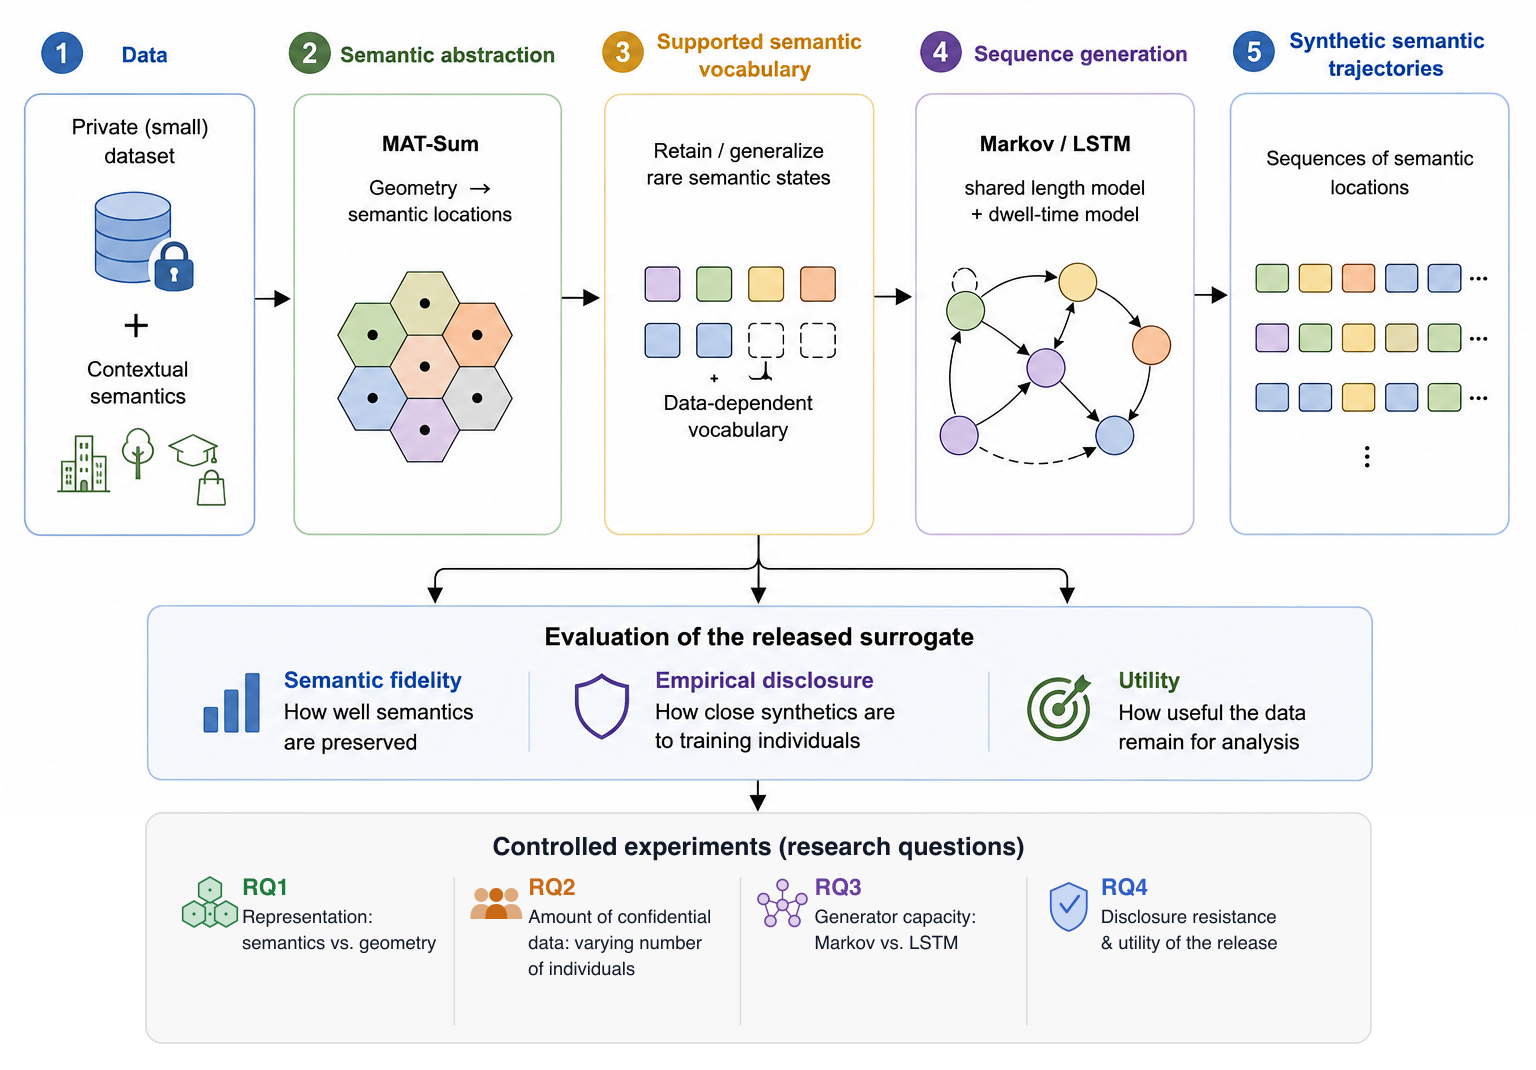
\includegraphics[width=\textwidth]{figures/methodology.png}
    \caption{
    Overview of the proposed methodology.
    %Confidential mobility data are first mapped by MAT-Sum to semantic
    %locations using a public OSM-based semantic map.
    %Rare semantic states are then generalized to obtain a
   % minimum-support, data-dependent vocabulary.
    %Synthetic semantic sequences are generated from this representation
    %using either an order-1 Markov model or an LSTM, while the empirical
   % sequence-length and dwell-time models are kept fixed.
    %Geographic re-materialization is optional and is not part of the
    %RQ1--RQ3 evaluation.
    }
    \label{fig:methodology}
\end{figure*}




\subsection{Problem setting and notation}
\label{sec:problem}

Let $\mathcal{U}$ denote a set of individuals moving into a geographical space. An individual
%$u \in \mathcal{U}$ 
contributes one or more trajectories, that are 
%
%\[
%    \mathcal{D}_u =
%    \left\{
%        X_{u,1}, \ldots, X_{u,R_u}
%    \right\},
%\]
%
%where
%
%\[
%    X_{u,r} =
%    \bigl[
%        (p_1,t_1),\ldots,(p_T,t_T)
%    \bigr]
%\]
%is a 
temporally ordered sequence of geographic observations.
%The complete dataset is
%
%\[
 %   \mathcal{D}
 %   =
 %   \bigcup_{u\in\mathcal{U}} \mathcal{D}_u .
%\]

%This notation covers both datasets used in our evaluation. A user may
%contribute a single aggregated trajectory or multiple recording
%sessions. Importantly, the \emph{individual} remains the sampling and
%privacy unit: sequences belonging to the same individual are never
%split across privacy comparisons.

In addition to the mobility data, we assume access to a
public semantic description of the study area, obtained, for example, from
OpenStreetMap (OSM) or similar public repositories. Let $\mathcal{L}$ denote the resulting common
vocabulary of semantic labels. This public label space is fixed within each study area and is used as a common evaluation space throughout the experiments.

\subsection{Semantic abstraction}
\label{sec:semantic-abstraction}

We use MAT-Sum~\cite{pugliese2023} to transform raw mobility observations into visits to semantically characterized locations. MAT-Sum tessellates the geographic area, enriches the resulting cells with semantic aspects, and groups cells that share a semantic context into semantic locations.

%For a semantic location $\ell$, let $\mathcal{A}(\ell)$ denote its set
%of semantic aspects. We represent $\ell$ through a compact signature
%obtained by retaining its top-$m$ TF--IDF-ranked aspects:
%
%\[
%    \phi_m(\ell)
%    =
%    \operatorname{Top}_m\!\left(\mathcal{A}(\ell)\right).
%\]
%
%The parameter $m$ therefore controls the semantic resolution of the
%representation: smaller values produce coarser signatures and a smaller
%state space, whereas larger values preserve finer semantic distinctions.

Each raw trajectory is mapped to the corresponding sequence of semantic
locations. Consecutive observations associated with the same semantic location
are run-length collapsed into a single visit, while their elapsed time
is accumulated as a dwell time. The resulting representation is
%
\[
    S_{u,r}
    =
    \bigl[
        (z_1,\delta_1),\ldots,(z_L,\delta_L)
    \bigr],
\]
%
where $z_i$ is a semantic state and $\delta_i$ its dwell time.

\subsection{Minimum-support semantic vocabulary}
\label{sec:vocabulary}

As we are in the scenario where we ned to create data driven synthetic data from small 9confidential) datasets, we have to consider that a vocabulary built from a small sample may contain rare semantic contexts that are weakly supported and potentially identifying the individual.
We therefore apply a minimum-support generalization controlled by a parameter $k$.

%Let
%
%\[
%    \operatorname{supp}(z)
%\]
%
%denote the number of occurrences of semantic state $z$ in the training
%sample. States satisfying
%
%\[
%    \operatorname{supp}(z) < k
%\]
%
%are merged into a sufficiently supported state with the most similar
%semantic signature. 
Similarity between two semantic locations is measured by
their Jaccard similarity.
%
%\[
%    J(z_i,z_j)
%    =
 %   \frac{|z_i\cap z_j|}
 %        {|z_i\cup z_j|}.
%\]
%
%Thus a rare state $z$ is mapped to
%
%\[
%    z^{\star}
%    =
%    \arg\max_{
%        z'\,:\,\operatorname{supp}(z')\geq k
%    }
%    J(z,z').
%\]

The resulting vocabulary is denoted by
%
\[
    \mathcal{V}_{m,k}(\mathcal{D}).
\]
%
A key property for the experiments in RQ2 and RQ3 is that this vocabulary is reconstructed from the individuals available in each training sample.
Consequently, its effective cardinality may grow with the amount of training data. The public semantic map remains fixed; only the data-dependent vocabulary and the generative model are re-estimated.

Unless otherwise stated, the experiments use $m=2$ and $k=5$.

\subsection{Sequence generation}
\label{sec:generation}

Given the semantic sequences induced by
$\mathcal{V}_{m,k}(\mathcal{D})$, we model separately
(i) sequence length, (ii) semantic-state transitions, and
(iii) dwell times. This decoupling ensures that the comparison between different sequence generators changes the transition model while keeping the remaining components fixed.

%\subsubsection{Order-1 Markov generator}

Our main generator is a first-order Markov chain over the semantic vocabulary. Let
%
\[
    C_{ij}
\]
%
be the number of observed transitions from state $i$ to state $j$ in
the training sequences. With Laplace smoothing, the transition
probability is
%
\[
    P(z_{t+1}=j \mid z_t=i)
    =
    \frac{C_{ij}+1}
         {\sum_{j'} C_{ij'} + |\mathcal{V}_{m,k}|}.
\]

The sequence length is sampled independently from the empirical distribution of training-sequence lengths. Dwell times are sampled from the empirical per-state dwell-time distribution. Thus, once a semantic sequence
%
\[
    \widetilde{S}
    =
    [\tilde z_1,\ldots,\tilde z_L]
\]
%
has been generated, each visit receives a newly sampled dwell time associated with its semantic state.

No transition is introduced across independent recording sessions.
When a user contributes multiple sessions, transition counts are accumulated within sessions and the sequence model is reset at each session boundary.

% TODO: specify explicitly how the initial state of a synthetic
% sequence is sampled (e.g., empirical initial-state distribution).

%\subsubsection{LSTM generator}

To study the effect of sequence-model capacity in RQ3, we use a lightweight LSTM as a higher-capacity alternative. The LSTM operates on
the same data-dependent semantic vocabulary and estimates
%
\[
    P_{\theta}
    (z_t \mid z_1,\ldots,z_{t-1}).
\]

The purpose of this comparison is to change the conditional model used to generate the semantic state sequence. Therefore, for each paired experimental run, Markov and LSTM receive the same training users, the same MAT-Sum vocabulary, and the same empirical length and dwell-time models.

The architecture and training hyperparameters used in each dataset are reported in Section~\ref{sec:experiments}.

% TODO: report the sampling temperature and stopping/early-stopping
% criterion if applicable.

\subsection{Controlled geometric abstractions}
\label{sec:baselines}

As stated in our RQ1, we want to isolate the effect of the representation. We therefore compare
MAT-Sum with two purely geometric abstractions while holding the sequence generator and state-space budget fixed: the grid cells and the spatial clustering. 

%\paragraph{Grid.}
In the grid representation, the study area is discretized into spatial grid cells, and each visited cell becomes a sequence state.
In the spatial clustering approach, the GPS observations are grouped through spatial $K$-means clustering, and the resulting clusters define the sequence states.

For every paired experimental sample, let
%
\[
    K_r
    =
    |\mathcal{V}_{m,k}(\mathcal{D}^{(r)})|
\]
%
be the effective number of MAT-Sum states. The geometric abstractions
are configured to produce the same state-space budget $K_r$.
All three representations are then coupled with the same order-1 Markov generator and the same sampling protocol.

This controlled design makes the semantic abstraction the important factor in RQ1: differences cannot be attributed to a larger state space or a more expressive sequence generator.

%\subsection{A common semantic evaluation space}
%\label{sec:common-space}

The three abstractions used to answer RQ1 have different native-state semantics. Moreover, in RQ2 and RQ3 the MAT-Sum vocabulary is rebuilt for each training sample and therefore changes with the number of available users. Direct comparison only in the native state spaces would consequently mix generation error with differences in the representation itself.

We therefore evaluate semantic fidelity in a common public OSM-label space $\mathcal{L}$. For each abstraction $A$, let
%
\[
    \pi_A :
    \mathcal{V}_A \rightarrow \mathcal{L}
\]
%
be the post-hoc mapping from an abstraction state to its corresponding OSM semantic label. The same mapping is applied to both real abstracted sequences and generated sequences. This allows every method to be compared against the same reference OSM-label sequences.

For a collection of sequences $D$, let
%
\[
    P_D^{(q)}
\]
%
denote the empirical distribution of contiguous $q$-grams. We measure the discrepancy between two distributions $P$ and $Q$ using total variation (TV) distance,
%
\[
    \operatorname{TV}(P,Q)
    =
    \frac{1}{2}
    \sum_x |P(x)-Q(x)|,
\]
%
where lower values indicate greater distributional fidelity.
Total Variation distance is particularly well-suited to our setting because it quantifies how faithfully the synthetic data reproduce the empirical semantic transition distribution in a common, fixed label space.

\subsubsection{Native-state generation fidelity}

For RQ1, we first measure how accurately the generator reproduces the transition distribution within each abstraction's own state space:
%
\[
    D_{\mathrm{native}}(A)
    =
    \operatorname{TV}
    \left(
        P_{\mathcal{D}_A}^{(2)},
        P_{\widetilde{\mathcal{D}}_A}^{(2)}
    \right),
\]
%
where $\mathcal{D}_A$ and $\widetilde{\mathcal{D}}_A$ are respectively the real and synthetic sequences represented under abstraction $A$.
Since the alphabet differs across abstractions, this metric is
interpreted only as a within-representation generation error.

%\subsubsection{Abstraction distortion}

To quantify how much semantic information is lost before generation, we compare the real trajectories after abstraction and projection back to OSM labels with the original OSM-label reference:
%
\[
    D_{\mathrm{abs}}(A)
    =
    \operatorname{TV}
    \left(
        P_{\mathcal{D}_{\mathrm{OSM}}}^{(2)},
        P_{\pi_A(\mathcal{D}_A)}^{(2)}
    \right).
\]

This quantity isolates the distortion introduced by the abstraction itself, independently of the generator.

%\subsubsection{Semantic generation fidelity}

The final semantic-generation error is
%
\[
    D_{\mathrm{gen}}^{(q)}(A)
    =
    \operatorname{TV}
    \left(
        P_{\mathcal{D}_{\mathrm{OSM}}}^{(q)},
        P_{\pi_A(\widetilde{\mathcal{D}}_A)}^{(q)}
    \right).
\]

For RQ1 and RQ2, the primary fidelity measure is the semantic bigram distance $D_{\mathrm{gen}}^{(2)}$. In RQ2, this fixed OSM-label space is particularly important because the native MAT-Sum vocabulary changes with sample size and native-state TV would therefore be measured against a moving alphabet.

For RQ3 we report both
%
\[
    D_{\mathrm{gen}}^{(2)}
    \qquad\text{and}\qquad
    D_{\mathrm{gen}}^{(3)}.
\]
%
The bigram metric measures first-order transition fidelity, whereas the trigram metric exposes higher-order sequential structure that an order-1 Markov model cannot represent explicitly. Reporting both avoids evaluating the Markov model only on the statistic that it directly estimates.

\subsection{Empirical disclosure measures}
\label{sec:privacy-metrics}

Our privacy analysis does not address a formal privacy attack framework, which will be the subject of future work, but we focus on the empirical record-level memorization. These measures quantify proximity to the training data while they do not constitute a formal differential-privacy guarantee.

\subsubsection{Exact copies}

A generated sequence is an exact copy if its complete semantic
state sequence is identical to a sequence in the corresponding
training set. For $N$ generated sequences,
%
\[
    C_{\mathrm{exact}}
    =
    \sum_{s\in\widetilde{\mathcal{D}}}
    \mathbb{I}
    \left[
        \exists x\in\mathcal{D}_{\mathrm{train}}:
        s=x
    \right].
\]
%
We report this quantity as the number of exact copies among
$N=200$ generated sequences.

Since the sequence unit differs across datasets (an aggregated
trajectory or a recording session), exact-copy counts are interpreted within each dataset rather than directly compared across datasets.

%\subsubsection{Near copies}
Exact identity may miss synthetic sequences that reproduce almost all of a training record. We therefore use MUITAS~\cite{petry2019} as a
semantic trajectory-similarity measure. For a generated sequence $s$,
define
%
\[
    q(s)
    =
    \max_{x\in\mathcal{D}_{\mathrm{train}}}
    \operatorname{MUITAS}(s,x).
\]
%
A sequence is considered a \textit{near-copy} when
%
\[
    q(s) \geq 0.95.
\]
%
The near-copy rate is
%
\[
    C_{\mathrm{near}}
    =
    \frac{1}{N}
    \sum_{s\in\widetilde{\mathcal{D}}}
    \mathbb{I}[q(s)\geq0.95].
\]

%\subsubsection{Distance to the closest real record}

For each synthetic sequence $s$, we define its distance to a training individual $u$ as
%
\[
    d(s,u)
    =
    1 -
    \max_{x\in\mathcal{D}_u}
    \operatorname{MUITAS}(s,x).
\]
%
The synthetic-to-training Distance to the Closest Record (DCR) is then
%
\[
    \operatorname{DCR}_{\mathrm{synth}}
    =
    \frac{1}{N}
    \sum_{s\in\widetilde{\mathcal{D}}}
    \min_{u\in\mathcal{U}_{\mathrm{train}}}
    d(s,u).
\]

To make this quantity interpretable, we compare it with a matched
real-to-real baseline. For a real sequence $x$ belonging to user $u$, we exclude all other sequences of that same user and compute
%
\[
    d_{\mathrm{real}}(x)
    =
    1-
    \max_{\substack{
        v\neq u\\
        y\in\mathcal{D}_v
    }}
    \operatorname{MUITAS}(x,y).
\]
%
When individuals contribute multiple sessions, distances are first averaged within each user and then across users, preventing heavily observed individuals from dominating the baseline.

Finally, we report
%
\[
    \Delta\operatorname{DCR}
    =
    \operatorname{DCR}_{\mathrm{synth}}
    -
    \operatorname{DCR}_{\mathrm{base}}.
\]
%
A positive value means that, according to the chosen semantic
similarity measure, synthetic records are on average farther from their closest training individual than real records are from other real individuals. A negative value indicates comparatively greater proximity to the training data.

\subsection{Experimental design}
\label{sec:experimental-design}

The three research questions are evaluated through controlled paired experiments.

\paragraph{RQ1: role of the abstraction.}
We vary the representation while controlling the generator and
state-space budget. Grid, spatial clustering, and MAT-Sum are evaluated on the same user samples, with matched numbers of states and the same order-1 Markov generator. We report native-state bigram TV, common-label abstraction distortion, semantic generation TV, and copy-based disclosure measures.

\paragraph{RQ2: small-data scaling.}
We fix MAT-Sum and the order-1 Markov generator and vary the number of training individuals. Within each replicate, user samples are nested,
%
\[
    \mathcal{D}_{n_1}^{(r)}
    \subset
    \mathcal{D}_{n_2}^{(r)}
    \subset \cdots,
\]
%
so that changes along the scaling curve reflect the addition of
individuals rather than unrelated sample composition. The MAT-Sum
vocabulary is rebuilt at every $n$. For this reason, quality is
evaluated in the fixed OSM-label space rather than by comparing native state distributions across different $n$.

\paragraph{RQ3: sequence model and privacy-fidelity trade-off.}
We fix the MAT-Sum representation and compare the order-1 Markov and LSTM generators on the same paired user samples. Both models share the same vocabulary, empirical length model, dwell-time model, and output size. We measure first-order semantic fidelity through bigram TV, higher-order fidelity through trigram TV, and disclosure through near-copy rate, exact copies, and $\Delta\operatorname{DCR}$.

Unless stated otherwise, each configuration generates $N=200$
synthetic sequences and is evaluated over 20 paired replicates.
We report means and 95\% confidence intervals. For direct paired
comparisons, significance is assessed on replicate-wise differences using paired sign-flip permutation tests. Bootstrap confidence intervals of paired effects are reported where appropriate. Dataset-specific sample sizes and preprocessing choices are given in Section~\ref{sec:experiments}.

%\paragraph{Scope of the evaluation.}
The research questions in this work concern the semantic sequence
generation stage, i.e., the part of the pipeline above the geographic re-materialization step. Any subsequent instantiation of a generated semantic state at a concrete map location does not enter the distributional or disclosure results reported for RQ1--RQ3.



\section{Experimental Validation}
\label{sec:experiments}
\subsection{Datasets and protocol}

We test the method on two complementary mobility datasets: Paris-OSM \cite{pugliese2025}  and Geolife \cite{geolife}.

\paragraph{Paris-OSM dataset}
The Paris dataset is obtained from the semantically enriched OSM mobility dataset of~\cite{pugliese2025}: raw GPS
traces are merged into one trajectory per de-identified OpenStreetMap contributor, i.e. we have 581
individuals, 1.57\,M points. The merging is per-user, so we will refer to per-trajectory metrics as per-person metrics. The user $ids$ are de-identified.
We ran MAT-Sum map-enrichment on this area (squares, zoom~17): 32{,}697 enriched tiles
$\rightarrow$ 18{,}554 semantic locations.

Paris-OSM is the main dataset where we run our evaluation.
To isolate the contribution of the abstraction itself, we reduce three abstractions of the
same data to the same number of states ($\sim$328) and feed each to an identical order-1 Markov
generator, so any difference is attributable to how the state space is built, not to the
generator. 
\textsc{Grid-Markov} uses spatial grid cells, \textsc{Cluster-Markov} uses KMeans spatial
clusters, as in graph-based approaches~\cite{kavalionak2026}, \textsc{MAT-Sum-Markov} uses the
$m{=}2,k{=}5$ semantic vocabulary (328 symbols). For a fair semantic comparison, every state is
additionally mapped, post-hoc, to the same OSM label vocabulary (its dominant aspect), and evaluated
against the ground-truth per-point label sequences.

\paragraph{Geolife dataset}
To test whether our three main findings survive a change of city, period, collection modality, and
record structure, we replicate the core experiments on the public GeoLife dataset~\cite{geolife}
(182 users, 18{,}670 GPS sessions, Beijing, 2007--2012), as a targeted external validation
rather than a full re-run. GeoLife is session-structured, so we keep three distinct levels: the user,
the session and points: transitions are
counted only within a session, the generator is reset at each session, and the sampling and privacy unit remains the user. 
We selected a Beijing study area
(bounding box $\mathrm{lat}\in[39.75,40.10]$, $\mathrm{lon}\in[116.00,116.80]$) and three filters: (1) a session is kept if $\ge80\%$ of its points lie in the box (outside points are then clipped); (2) a session is valid if it has $\ge10$ semantic visits after run-length collapsing (not $10$ raw GPS
points); (3) a user is kept if it has $\ge3$ valid sessions. The semantic enrichment is identical to Paris-OSM (same OSM taxonomy, tessellation, aspects, $m{=}2,k{=}5$); the MAT-Sum vocabulary is, as in RQ2 and RQ3, rebuilt on the users of each sample.


\subsubsection*{GeoLife study-area audit and retention}
\label{sec:geolife-audit}

In this additional validation, we want to evaluate how the approach is still valid in another geographical area with a different mobility dataset, so we run a subset of the RQs experiments in the Geolife dataset.  

Each research question is additionally re-examined on GeoLife as an external replication, reported under RQ1--RQ3 below; here we first describe the GeoLife study area and the data these replications use.

We first present an analysis of experimental data for Geolife.

Table~\ref{tab:geolife-audit} reports the step-by-step retention. The filters are gentle---no stage
collapses the dataset, leaving $U{=}152$ effective users, $13{,}370$ valid sessions and
$16.8$\,M points. Semantic coverage is excellent: $99.4\%$ of the retained points fall in an enriched
cell ($0.6\%$ carry no label), over $40{,}620$ enriched cells, $11{,}050$ semantic locations and $65$
distinct OSM labels; the median user has $30$ valid sessions and $1{,}868$ semantic visits.
Figure~\ref{fig:geolife-diag} confirms the sample is not deformed: a broad, imbalanced
sessions-per-user distribution (justifying user-balanced training), semantically rich sessions, and a
spatially coherent study area centred on the GeoLife collection region. The stop conditions are
comfortably met, so we proceed. The audit fixes the scaling grid: $n{=}100$ for the
role-of-abstraction replication, $n\in\{10,20,30,50,75,100,150,152\}$ for the scaling study, and
$n\in\{20,50,100,152\}$ for the Markov--LSTM comparison.

\begin{table}[t]
  \caption{GeoLife retention under the frozen filters (Beijing study box). No cross-session
  concatenation; unit $=$ user. Users, sessions and points surviving each successive step.}
  \label{tab:geolife-audit}
  \small
  \begin{tabular}{@{}lrrr@{}}
    \toprule
    step & users & sessions & points \\
    \midrule
    GeoLife original            & 182 & 18{,}670 & 24{,}876{,}978 \\
    $\ge1$ point in box         & 179 & 17{,}156 & 18{,}695{,}336 \\
    $\ge80\%$ in box (clipped)  & 173 & 16{,}343 & 17{,}261{,}196 \\
    $\ge10$ semantic visits     & 169 & 13{,}393 & 16{,}889{,}348 \\
    $\ge3$ valid sessions/user  & \textbf{152} & \textbf{13{,}370} & \textbf{16{,}849{,}399} \\
    \bottomrule
  \end{tabular}
\end{table}

\begin{figure*}[t]
  \centering
  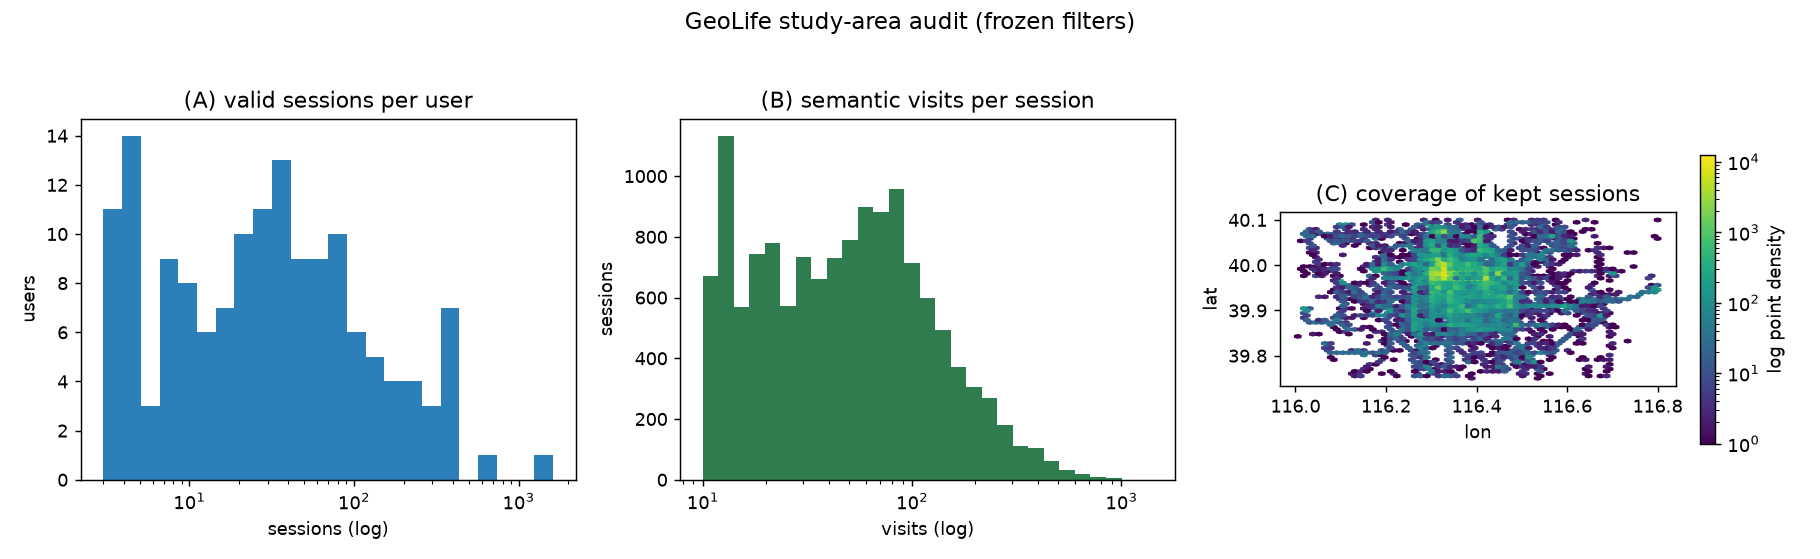
\includegraphics[width=\textwidth]{figures/fig_geolife_diag.png}
  \caption{GeoLife pre-experiment audit (frozen filters). \textbf{(A)}~valid sessions per user (broad,
  imbalanced---some users dominate, motivating user-balanced training); \textbf{(B)}~semantic visits
  per session (rich; the $\ge10$ cut removes only the short left tail); \textbf{(C)}~spatial coverage
  of the kept sessions---a coherent area centred on the GeoLife collection region, not scattered
  points.}
  \label{fig:geolife-diag}
\end{figure*}

\subsection{RQ1 - The role of the semantic abstraction}
\label{sec:abstraction}


Table~\ref{tab:abstraction} and Figure~\ref{fig:abstraction} show that the controlled comparison supports two complementary observations. As expected, an abstraction explicitly constructed from semantic context preserves OSM-level semantics better than purely geometric alternatives. More importantly, this advantage is not limited to the semantic evaluation space: under the same state budget and the same Markov generator, MAT-Sum also yields substantially lower generation error within its own native state space. This suggests that semantic abstraction not only preserves the target information, but also organizes mobility into a transition space that is easier to model.
In Table ~\ref{tab:abstraction}, three abstractions are reduced to approximately 328 states and coupled with the same first-order Markov generator. Values are means and 95\% confidence intervals over the same 20 paired user samples used in Fig. \ref{fig:abstraction}. Metrics are grouped by measurement space: bigram TV is evaluated within each representation’s native state space, whereas distortion and generation TV are evaluated against the same OSM-label ground truth. Copies denote the mean number of generated state sequences that exactly match a sequence in the corresponding sampled real training set, per run, out of N=200 synthetic trajectories. 
We can notice the following facts: 
(i)~It roughly halves the generic state-level bigram-TV (0.32 vs.\
0.59--0.62): semantically-defined states induce more regular, learnable transitions than arbitrary
spatial ones. (ii)~It loses far less structure to the abstraction itself - the semantic
distortion (real states mapped back to labels vs.\ ground truth) is 0.28 against 0.47--0.54,
because a spatial cell inevitably mixes distinct semantic contexts, whereas a \textsc{MAT-Sum} state is
semantically coherent by construction. (iii)~Its synthetic data reproduces the real semantic label-transition distribution markedly better (0.27 vs.\ 0.43--0.46). It is also the safest (no exact copies, against 1 and 9), and, uniquely, its states are interpretable, multi-aspect locations rather than anonymous cell or cluster ids. The role of MAT-Sum is thus neither the state count nor the generator: building the state space from semantics preserves structure that spatial abstractions cannot represent at the same resolution.

As expected from its semantic construction, MAT-Sum introduces substantially less semantic distortion than purely geometric abstractions.

\begin{table*}[t]
  \caption{Role of the abstraction on Paris-OSM. All quantities are lower-is-better. }
  \label{tab:abstraction}
  \small
  \begin{tabular}{@{}lccccc@{}}
    \toprule
    & native space & \multicolumn{2}{c}{common-label space} & & privacy \\
    \cmidrule(lr){2-2}\cmidrule(lr){3-4}\cmidrule(lr){6-6}
    abstraction & bigram TV & distortion & gen-TV & & copies \\
    \midrule
    Grid-Markov                          & $0.652\pm0.010$ & $0.548\pm0.004$ & $0.484\pm0.007$ & & $4.9\pm1.3$ \\
    Cluster-Markov~\cite{kavalionak2026} & $0.656\pm0.008$ & $0.475\pm0.003$ & $0.441\pm0.006$ & & $2.3\pm0.7$ \\
    \textsc{MAT-Sum}-Markov              & $\mathbf{0.362\pm0.004}$ & $\mathbf{0.282\pm0.003}$ & $\mathbf{0.279\pm0.002}$ & & $\mathbf{0.2\pm0.2}$ \\
    \bottomrule
  \end{tabular}
\end{table*}

\begin{figure*}[t]
  \centering
  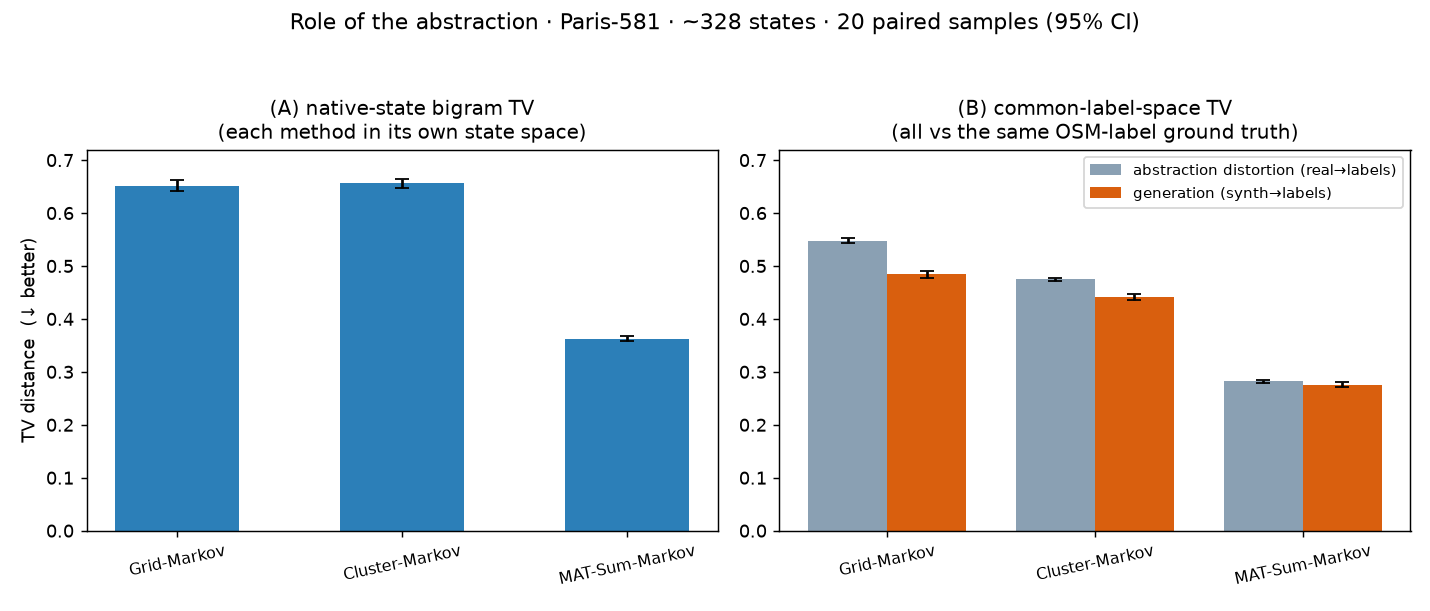
\includegraphics[width=\textwidth]{figures/fig_abstraction_ci.png}
  \caption{Role of the abstraction (Paris-OSM, $\sim$328 states, same order-1 Markov; means over 20
  paired user samples, 95\% CI). \textbf{(A)}~Native-state bigram TV: each method is compared against
  its \emph{own} $\sim$328-state real distribution, so the reference differs across methods (grid
  cells, clusters, or semantic symbols) even though the metric is a TV. \textbf{(B)}~Common-label-space
  TV: every method is mapped to the same OSM-label ground truth and compared on it - abstraction
  distortion (real states $\to$ labels) and generation fidelity (synthetic states $\to$ labels). The
  two panels, therefore, measure different objects and must not be read across; within each, the
 semantic abstraction (\textsc{MAT-Sum}) is significantly better.}
  \label{fig:abstraction}
\end{figure*}

%The abstraction matters: under the same Markov generator and a comparable number of states, the MAT-Sum representation halves the native bigram discrepancy and substantially reduces semantic distortion.

%We run this paired test:
%$d_i \;=\; \mathrm{TV}_{i,\text{baseline}} %\;-\; \mathrm{TV}_{i,\text{MAT\text{-}Sum}}$

\begin{table}[t]
  \caption{Paired per-sample improvement $d_i=\mathrm{TV}_{i,\text{baseline}}-\mathrm{TV}_{i,\text{\textsc{MAT-Sum}}}$
  over $R{=}20$ paired user samples (positive $=$ \textsc{MAT-Sum} better). Mean (median), bootstrap 95\%
  CI, paired effect size Cohen's $d_z$, and an exact paired sign-flip permutation test.}
  \label{tab:paired}
  \small
  \begin{tabular}{@{}llccc@{}}
    \toprule
    baseline & metric & $\bar d$ (med.) & 95\% CI & $d_z$ \\
    \midrule
    Grid    & generic bi-TV     & $0.290\,(0.291)$ & $[0.281,0.299]$ & $14.2$ \\
    Grid    & sem.\ distortion  & $0.266\,(0.266)$ & $[0.263,0.270]$ & $30.1$ \\
    Grid    & sem.\ gen-TV      & $0.204\,(0.206)$ & $[0.197,0.211]$ & $13.1$ \\
    Cluster & generic bi-TV     & $0.293\,(0.295)$ & $[0.286,0.300]$ & $18.0$ \\
    Cluster & sem.\ distortion  & $0.193\,(0.193)$ & $[0.191,0.196]$ & $35.9$ \\
    Cluster & sem.\ gen-TV      & $0.162\,(0.164)$ & $[0.156,0.168]$ & $12.2$ \\
    \bottomrule
  \end{tabular}
  \\[2pt]\footnotesize All differences: permutation and Wilcoxon $p<10^{-4}$; Shapiro $p>0.05$.
\end{table}

For each paired sample $i$ we take $d_i=\mathrm{TV}_{i,\text{baseline}}-\mathrm{TV}_{i,\textsc{MAT-Sum}}$.
Across $R{=}20$ samples every $d_i$ is positive with a tight bootstrap 95\% CI excluding zero
(Table~\ref{tab:paired}); an exact paired sign-flip permutation test gives $p<10^{-4}$ (Wilcoxon
signed-rank agrees), and the paired effect size is very large (Cohen's $d_z>12$). The advantage of
the semantic abstraction is therefore statistically robust rather than an artifact of a particular split.

%\subsection{Summarization at scale (context for RQ1)}
%On Paris-581, \textsc{MAT-Sum} attains a dataset summarization rate $S_{\text{rate}}=0.921$
%(per-individual range 0.45--0.996), within the published Geolife range (0.90--0.98). The
%proof-of-concept's lower 0.738 was not a method weakness but data sparsity---the PoC trajectories are
%short (84--481 points) while the validation trajectories are densely sampled---confirming that dense
%semantic trajectories compress into few semantic locations very effectively.

%\subsection{Granularity, fidelity and privacy (RQ2)}
%Table~\ref{tab:sweep} sweeps the $(m,k)$ dial on Paris-581 ($N=200$ synthetic; nearest-neighbor over a
%150-sample). At every setting the mechanistic generator's DCR sits at or above the real-to-real
%baseline---it is never closer to real records than real records are to one another---and verbatim
%copies are essentially absent. Increasing $k$ both anonymizes and, by densifying the alphabet,
%improves fidelity; the vocabulary grows with the city ($m{=}3\rightarrow959$ symbols, versus 71 on the
%small PoC), so fine granularity remains sparse even at $n{=}581$, motivating the scaling study.

%\begin{table*}[t]
%\caption{$(m,k)$ sweep on Paris-581. $\downarrow$ lower is better, $\uparrow$ higher is better.}
%\label{tab:sweep}
%\small
%\begin{tabular}{@{}rrrrrrrrr@{}}
%\toprule
%$m$ & $k$ & alphabet & unigram TV\,$\downarrow$ & bigram TV\,$\downarrow$ &
%MUITAS$\rightarrow$real\,$\uparrow$ & DCR\,$\uparrow$ & DCR base & copies \\
%\midrule
%1 & 5 & 52   & 0.021 & 0.097 & 0.913 & 0.087 & 0.079 & 2 \\
%2 & 5 & 328  & 0.134 & 0.329 & 0.630 & 0.370 & 0.253 & 0 \\
%3 & 5 & 959  & 0.342 & 0.716 & 0.402 & 0.598 & 0.350 & 0 \\
%2 & 2 & 441  & 0.211 & 0.412 & 0.571 & 0.429 & 0.274 & 1 \\
%3 & 2 & 1410 & 0.463 & 0.830 & 0.346 & 0.654 & 0.388 & 0 \\
%\bottomrule
%\end{tabular}
%\end{table*}

\subsubsection*{External replication (GeoLife)}
\label{sec:geolife-e1}


We test whether the advantage of semantic abstraction generalizes beyond Paris. We replicate the controlled comparison for RQ1 on GeoLife using 20 paired samples, each with n=100 users. For each sample, the MAT-Sum vocabulary is rebuilt from the selected users and its effective number of states $K_r$
 is recorded. Grid and spatial-clustering abstractions are then configured to produce the same $K_r$, approximately 594 states on average. All representations are coupled with the same order-1 Markov generator, session-length model, and sampling protocol, producing N=200 synthetic sessions per run. Since GeoLife contains multiple sessions per user, transitions are counted only within sessions and the generator is reset at every session boundary.

 Table~\ref{tab:geolife-e1} and
Figure~\ref{fig:geolife-e1} show the Paris result replicates cleanly: the semantic abstraction is best on every axis with non-overlapping 95\% CIs, native-state bigram TV, semantic distortion, semantic generation, and both privacy measures. The gap is, if anything, sharper on privacy: at the matched state
count the grid produces $31.8$ exact session copies out of $200$ (short Beijing sessions collide in a coarse cell grid) and a $76\%$ near-copy rate, against $0$ exact copies and $21\%$ for MAT-Sum. The role of the semantic abstraction therefore survives the change of city, period, collection modality
and record structure.

\begin{table*}[t]
  \caption{GeoLife (RQ1; $n{=}100$, 20 paired samples, $K_r{\approx}594$ matched states). Mean $\pm$
  95\% CI; TV$\downarrow$; copies out of $N{=}200$; near-copy at common-label MUITAS $\ge0.95$.}
  \label{tab:geolife-e1}
  \small
  \begin{tabular}{@{}lccccc@{}}
    \toprule
    & native bi-TV & \multicolumn{2}{c}{common-label space} & \multicolumn{2}{c}{privacy} \\
    \cmidrule(lr){2-2}\cmidrule(lr){3-4}\cmidrule(lr){5-6}
    method & bigram TV & distortion & gen-TV & exact/200 & near-copy \% \\
    \midrule
    Grid                          & $0.389\pm0.011$ & $0.636\pm0.026$ & $0.613\pm0.027$ & $31.8\pm2.4$ & $76.2\pm1.9$ \\
    Cluster~\cite{kavalionak2026} & $0.381\pm0.008$ & $0.421\pm0.012$ & $0.419\pm0.012$ & $1.6\pm0.5$  & $61.1\pm3.4$ \\
    \textsc{MAT-Sum}              & $\mathbf{0.259\pm0.004}$ & $\mathbf{0.175\pm0.006}$ & $\mathbf{0.266\pm0.005}$ & $\mathbf{0.0\pm0.0}$ & $\mathbf{21.1\pm2.3}$ \\
    \bottomrule
  \end{tabular}
\end{table*}

\begin{figure*}[t]
  \centering
  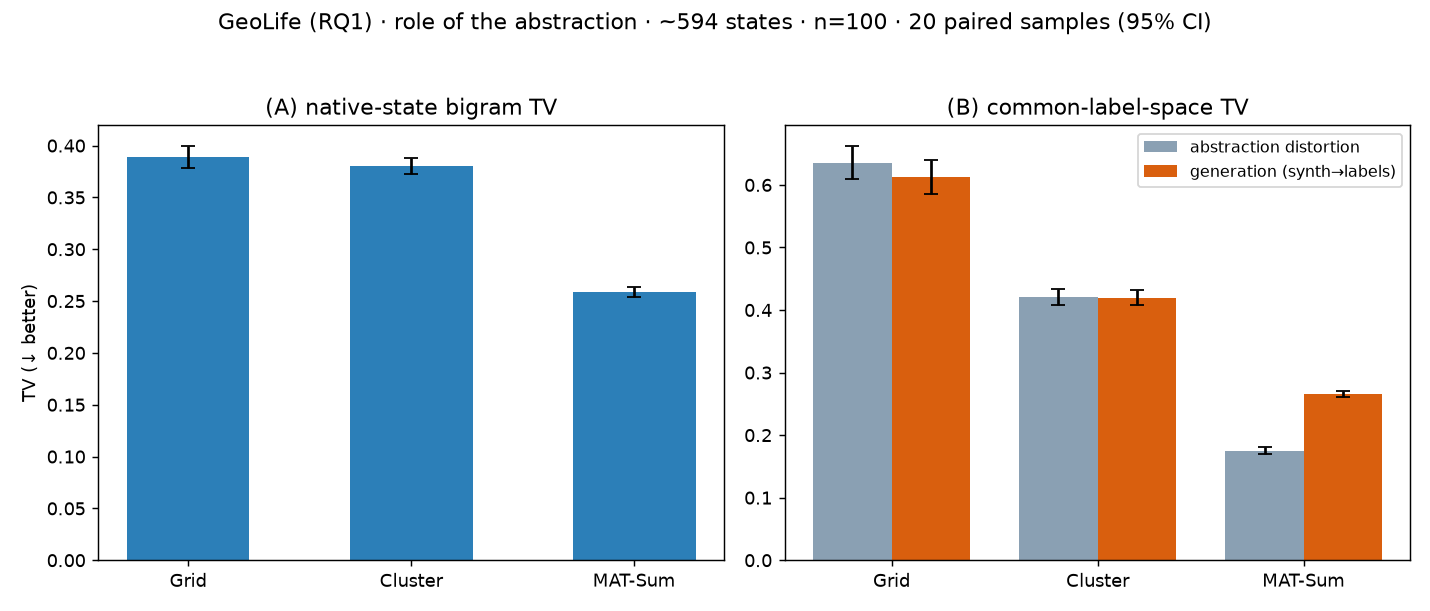
\includegraphics[width=\textwidth]{figures/fig_geolife_e1.png}
  \caption{GeoLife (RQ1): role of the abstraction at matched state count ($K_r{\approx}594$),
  $n{=}100$, 20 paired samples. \textbf{(A)}~native-state bigram TV; \textbf{(B)}~common-label-space
  TV (distortion, generation). \textsc{MAT-Sum} is significantly best in both spaces, replicating the
  Paris finding; whiskers are 95\% CIs.}
  \label{fig:geolife-e1}
\end{figure*}


 MAT-Sum achieves the lowest native-state bigram TV (0.259), compared with 0.389 for the grid and 0.381 for spatial clustering. Its advantage is even larger in the common semantic-label space: abstraction distortion decreases to 0.175, against 0.421–0.636, while semantic generation TV falls to 0.266, against 0.419–0.613. These results indicate that semantic locations are not only more coherent representations of the original data, but also define a transition space that can be learned more accurately by the same sequence generator.

MAT-Sum also exhibits substantially less record-level reproduction than the matched geometric abstractions. It produces no exact training-session copies, compared with 1.6 copies per 200 synthetic sessions for clustering and 31.8 for the grid. Its near-copy rate is also markedly lower, although still non-negligible on GeoLife: 21.1\%, compared with 61.1\% and 76.2\%. We therefore interpret this as evidence that semantic abstraction strongly reduces memorization relative to geometric representations, rather than as a standalone guarantee of privacy. Overall, the role of MAT-Sum survives the change of city, period, data-collection modality, and record structure.


\subsection{RQ2 - Small-data scaling and memorization}

We now test how our approach addresses RQ2 on data scaling.

In Figure \ref{fig:rq2} we report the plots for 
\textsc{MAT-Sum}$+$order-1 Markov, $m{=}2,k{=}5$; 20 nested paired replicates $D_{20}\!\subset\!D_{50}\!\subset\!D_{100}\!\subset\!D_{300}\!\subset\!D_{581}$; fixed abstraction parameters). \textbf{(A)}~quality (semantic generation TV) improves steadily with the number of individuals $n$. \textbf{(B)}~synthetic-to-training DCR meets or exceeds the per-sample real-to-real baseline for $n\ge50$. MAT-Sum also yields the lowest exact-copy count, averaging 0.2 copies per 200 synthetic sequences, compared with 2.3 for Cluster-Markov and 4.9 for Grid-Markov.
  

\begin{figure*}[t]
  \centering
  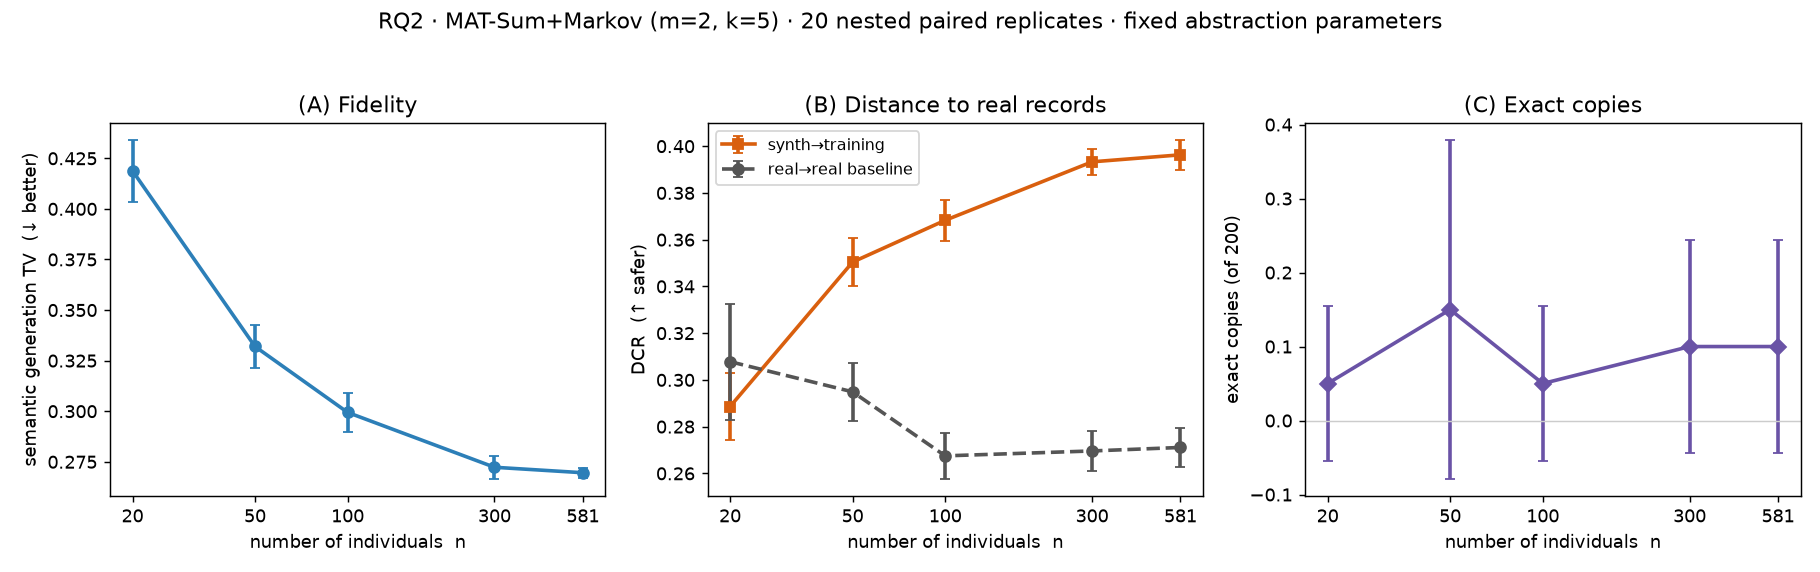
\includegraphics[width=\textwidth]{figures/fig_rq2.png}
  \caption{RQ2 on Paris-OSM}
  \label{fig:rq2}
\end{figure*}

\begin{table*}[t]
  \caption{RQ2 (Paris-OSM, \textsc{MAT-Sum}$+$order-1 Markov, $m{=}2,k{=}5$; 20 nested paired
  replicates, fixed abstraction parameters). Mean $\pm$ 95\% CI. $\Delta\mathrm{DCR}=
  \mathrm{DCR}_{\text{synth}}-\mathrm{DCR}_{\text{base}}$; copies out of $N{=}200$.}
  \label{tab:rq2}
  \small
  \begin{tabular}{@{}rccccc@{}}
    \toprule
    $n$ & sem.\ gen-TV\,$\downarrow$ & exact copies & DCR synth\,$\uparrow$ & DCR base & $\Delta$DCR \\
    \midrule
    20  & $0.419\pm0.015$ & $0.05\pm0.10$ & $0.289\pm0.015$ & $0.308\pm0.025$ & $-0.019\pm0.019$ \\
    50  & $0.332\pm0.011$ & $0.15\pm0.23$ & $0.350\pm0.010$ & $0.295\pm0.013$ & $+0.055\pm0.013$ \\
    100 & $0.299\pm0.010$ & $0.05\pm0.10$ & $0.368\pm0.009$ & $0.268\pm0.010$ & $+0.101\pm0.011$ \\
    300 & $0.272\pm0.006$ & $0.10\pm0.14$ & $0.393\pm0.006$ & $0.270\pm0.009$ & $+0.124\pm0.009$ \\
    581 & $0.270\pm0.003$ & $0.10\pm0.14$ & $0.396\pm0.006$ & $0.271\pm0.008$ & $+0.125\pm0.010$ \\
    \bottomrule
  \end{tabular}
\end{table*}


\begin{table}[t]
  \caption{Representation diagnostics vs.\ $n$ (means over 20 replicates): the effective state space
  and the transition support grows with the number of individuals, explaining the quality gain.}
  \label{tab:rq2diag}
  \small
  \begin{tabular}{@{}rccc@{}}
    \toprule
    $n$ & effective states & observed bigrams & median support/state \\
    \midrule
    20  & 68  & 644  & 11.7 \\
    50  & 119 & 1390 & 14.1 \\
    100 & 170 & 2281 & 16.1 \\
    300 & 267 & 4313 & 23.3 \\
    581 & 328 & 5963 & 29.4 \\
    \bottomrule
  \end{tabular}
\end{table}

As the number of available individuals increases, semantic fidelity improves steadily (semantic
generation TV $0.42\!\to\!0.27$). Exact sequence copying remains negligible at every $n$ ($\le0.15$ of $200$), and the synthetic-to-training DCR meets or exceeds the matched per-sample
real-to-real baseline for $n\ge50$ ($\Delta\mathrm{DCR}>0$), being only marginally below it at the extremely small sample $n{=}20$ ($\Delta\mathrm{DCR}=-0.019\pm0.019$). Empirical record-level memorization, therefore, remains limited across the studied data regimes.


Semantic generation quality improves monotonically as the number of training individuals increases: generation TV in the fixed OSM-label space decreases from approximately 0.42 at n=20 to 0.27 at n=581, with narrow confidence intervals and diminishing gains beyond n=300. Native-state bigram TV is not used for this comparison because the vocabulary is reconstructed for each sample and expands from 68 to 328 states, making its reference distribution dependent on n. Diagnostic statistics explain the semantic improvement: the number of observed bigrams grows from 644 to 5,963, while median state support rises from 12 to 29, yielding richer and better-supported transition estimates.

Empirical record-level disclosure remains limited. Exact copying is negligible throughout, averaging 0.15 copies per 200 generated trajectories. At n=20, the synthetic-to-training DCR is approximately equal to the matched real-to-real baseline $(\Delta DCR=-0.019 \pm 0.019)$. From n=50 onward, the margin becomes positive, and increases from approximately $+0.055$ to $+0.125$, indicating that synthetic trajectories become more distant from individual training records than real records are from one another.


In summary, additional individuals improve semantic fidelity and model support without increasing exact memorization. Beyond the smallest regime, they also increase the separation between synthetic trajectories and individual training records.

\subsubsection*{External replication (GeoLife)}
\label{sec:geolife-e2}

We examine how generation quality and empirical disclosure risk evolve as the number of available users increases. We construct 20 nested user samples for n$\in${10,20,30,50,75,100,150,152}. At each value of n, the MAT-Sum vocabulary, order-1 Markov model, and empirical session-length model are estimated exclusively from the selected users, while the public map and semantic enrichment remain fixed. The main quality measure is semantic generation TV in the common OSM-label space. Disclosure is evaluated through exact session copies and a user-aware DCR, in which each synthetic session is compared with the closest session belonging to any training user, while the real-to-real baseline excludes sessions from the same individual.


Table~\ref{tab:geolife-e2} and Figure~\ref{fig:geolife-e2} show that the direction replicates,  but the magnitude is smaller: quality improves monotonically yet gently ($0.273\!\to\!0.249$, a $9\%$
reduction against $36\%$ on Paris), with an estimated scaling breakpoint $n^\star\!\approx\!75$ (95\% CI
$[20,100]$; segmented fit of TV vs.\ $\log n$, bootstrapped over replicates). The reason is that GeoLife
individuals are information-rich (a median of $30$ sessions and $\sim$1868 semantic visits each), so the generator is already competent at $n{=}10$ and saturates early, scaling behaviour is governed by the information per individual, not merely their number. Disclosure risk again stays limited: exact session copies are $0$ at every $n$, and the user-aware $\Delta$DCR is marginally negative only at $n{=}10$
($-0.021\pm0.016$), turning positive for $n\ge20$ and widening to $+0.038$ as the real-to-real baseline
falls with $n$ while the synthetic distance holds.

\begin{table*}[t]
  \caption{GeoLife (RQ2; MAT-Sum$+$Markov, 20 nested paired replicates). Mean $\pm$ 95\% CI;
  $\Delta$DCR $=\mathrm{DCR}_{\text{synth}}-\mathrm{DCR}_{\text{base}}$ (user-aware); copies out of $200$.}
  \label{tab:geolife-e2}
  \small
  \begin{tabular}{@{}rccccc@{}}
    \toprule
    $n$ & sem.\ gen-TV\,$\downarrow$ & exact/200 & DCR synth\,$\uparrow$ & DCR base & $\Delta$DCR \\
    \midrule
    10  & $0.273\pm0.014$ & $0.0$ & $0.235\pm0.014$ & $0.256\pm0.014$ & $-0.021\pm0.016$ \\
    20  & $0.283\pm0.018$ & $0.0$ & $0.252\pm0.011$ & $0.246\pm0.014$ & $+0.006\pm0.015$ \\
    30  & $0.281\pm0.017$ & $0.0$ & $0.259\pm0.009$ & $0.236\pm0.010$ & $+0.023\pm0.012$ \\
    50  & $0.279\pm0.014$ & $0.0$ & $0.252\pm0.009$ & $0.223\pm0.009$ & $+0.029\pm0.012$ \\
    75  & $0.277\pm0.008$ & $0.0$ & $0.249\pm0.007$ & $0.216\pm0.007$ & $+0.033\pm0.006$ \\
    100 & $0.267\pm0.007$ & $0.0$ & $0.249\pm0.008$ & $0.211\pm0.006$ & $+0.038\pm0.009$ \\
    150 & $0.255\pm0.006$ & $0.0$ & $0.240\pm0.007$ & $0.205\pm0.006$ & $+0.035\pm0.006$ \\
    152 & $0.249\pm0.005$ & $0.0$ & $0.239\pm0.005$ & $0.206\pm0.005$ & $+0.033\pm0.004$ \\
    \bottomrule
  \end{tabular}
\end{table*}

\begin{figure*}[t]
  \centering
  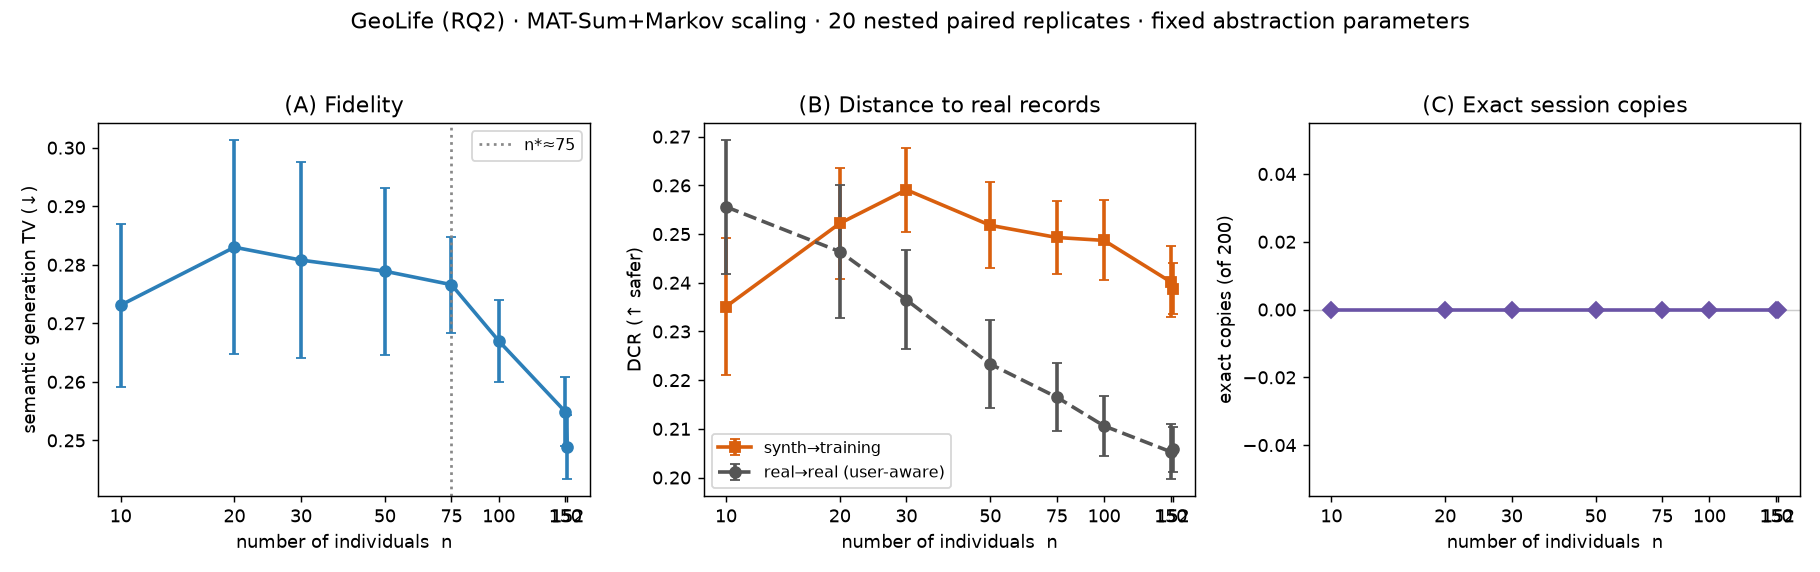
\includegraphics[width=\textwidth]{figures/fig_geolife_e2.png}
  \caption{GeoLife (RQ2) scaling, 20 nested paired replicates. \textbf{(A)}~semantic generation TV
  improves gently with $n$ (estimated saturation $n^\star\!\approx\!75$, dotted); \textbf{(B)}~user-aware
  DCR: synthetic$\to$training meets/exceeds the real-to-real baseline for $n\ge20$; \textbf{(C)}~exact
  session copies are $0$ throughout. Means $\pm$ 95\% CI.}
  \label{fig:geolife-e2}
\end{figure*}

Semantic fidelity shows an overall improvement as additional users become available, although the curve contains small-sample fluctuations. Semantic generation TV changes from 0.273 at n=10 to 0.249 at n=152, corresponding to an overall reduction of approximately 9\%. The gain is less pronounced than in Paris, and the fitted curve suggests a change in scaling behavior around n~75. Rather than indicating a universal sample-size threshold, this result reflects the information-rich structure of GeoLife: the median retained user contributes 30 sessions and approximately 1,868 semantic visits. Consequently, even a small number of users provides a substantial number of observations and transitions, and the marginal value of additional users is smaller than in Paris.

Empirical disclosure remains limited throughout the scaling experiment. No exact session copies are observed at any value of n. The user-aware $\Delta$DCR is slightly negative at n=10, -0.021$\pm$ 0.016, indicating that synthetic sessions are marginally closer to the training data than the matched real-to-real baseline. From n=20 onward, however, the margin becomes positive and remains so, reaching approximately +0.03$\pm$0.04 in the larger regimes. Taken together with the Paris results, this replication suggests that generation quality depends not only on the number of individuals but also on the amount and diversity of mobility information contributed by each individual.

Under an identical segmented log-$n$ fit the Paris saturation point is $n^\star{=}50$
(95\% CI $[50,100]$), statistically indistinguishable from GeoLife's $n^\star{=}75$ $[20,100]$:
the datasets differ in the \emph{magnitude} of the pre-plateau gain, not in where quality saturates.

\subsection{RQ3 - Generator capacity and privacy–fidelity trade-off}
\label{sec:rq3}

RQ3 asks whether, at a fixed \textsc{MAT-Sum} representation, increasing generator capacity buys better semantic fidelity, and at what disclosure cost. We compare two generators: the order-1 Markov and a small LSTM language model over the same per-sample symbol vocabulary holding everything else identical: the same nested paired user samples as RQ2
($D_{20}\!\subset\!D_{50}\!\subset\!D_{100}\!\subset\!D_{300}\!\subset\!D_{581}$, 20 replicates),
$m{=}2,k{=}5$, the same empirical length distribution, the same dwell model, and $N{=}200$ synthetic
trajectories per run. We report three quantities per $(n,\text{model})$: the \emph{semantic
generation TV} (quality in the fixed OSM-label space); the \emph{near-copy rate}, i.e.\ the fraction
of the $200$ synthetic trajectories whose maximum MUITAS similarity to any training individual is
$\ge0.95$ (the central empirical-disclosure metric); and
$\Delta\mathrm{DCR}=\mathrm{DCR}_{\text{synth}}-\mathrm{DCR}_{\text{base}}$ against the matched
per-sample real-to-real baseline. Exact copies are recorded as a secondary measure.

Table~\ref{tab:rq3} and Figure~\ref{fig:rq3} give a consistent answer: additional capacity does not help. On semantic fidelity, the Markov is better than the LSTM at every $n$, with non-overlapping confidence intervals (e.g.\ $0.421\pm0.015$ vs.\ $0.483\pm0.013$ at $n{=}20$, and $0.271\pm0.002$ vs.\
$0.314\pm0.006$ at $n{=}581$): the small LSTM under-models the semantic transition structure that the first-order chain captures directly. On disclosure risk, the LSTM is worse: its near-copy rate reaches
$3.5\%$ at $n{=}20$ against $0.1\%$ for the Markov  - a $\sim$35-fold gap - decaying to comparable values only for $n\ge300$, and its $\Delta\mathrm{DCR}$ is lower (less safe) at every $n$, crossing from negative to positive only at $n{=}100$ where the Markov already does so by $n{=}50$. Both effects are
sharpest in the small-data regime that motivates the work.

The same trade-off holds in Paris: the LSTM lowers the trigram TV at every $n$
(paired sign-flip test, Markov$-$LSTM $=+0.018$ to $+0.049$, all $p<10^{-3}$): its extra
capacity captures higher-order sequential structure, the memoryless chain cannot, yet it
does so at the cost of worse first-order fidelity and higher record-level disclosure, so the order-1 Markov remains the preferred operating point for privacy-preserving synthesis.


\emph{Summary.} At a fixed \textsc{MAT-Sum} representation, the order-1 Markov
performs better than the deep LSTM on both quality and record-level disclosure risk across all studied data
regimes. Extra capacity trades no fidelity gain for measurably higher memorization, most acutely when individuals are scarce. 
We therefore adopt the order-1 Markov as the generator in the remainder.



\begin{figure*}[t]
  \centering
  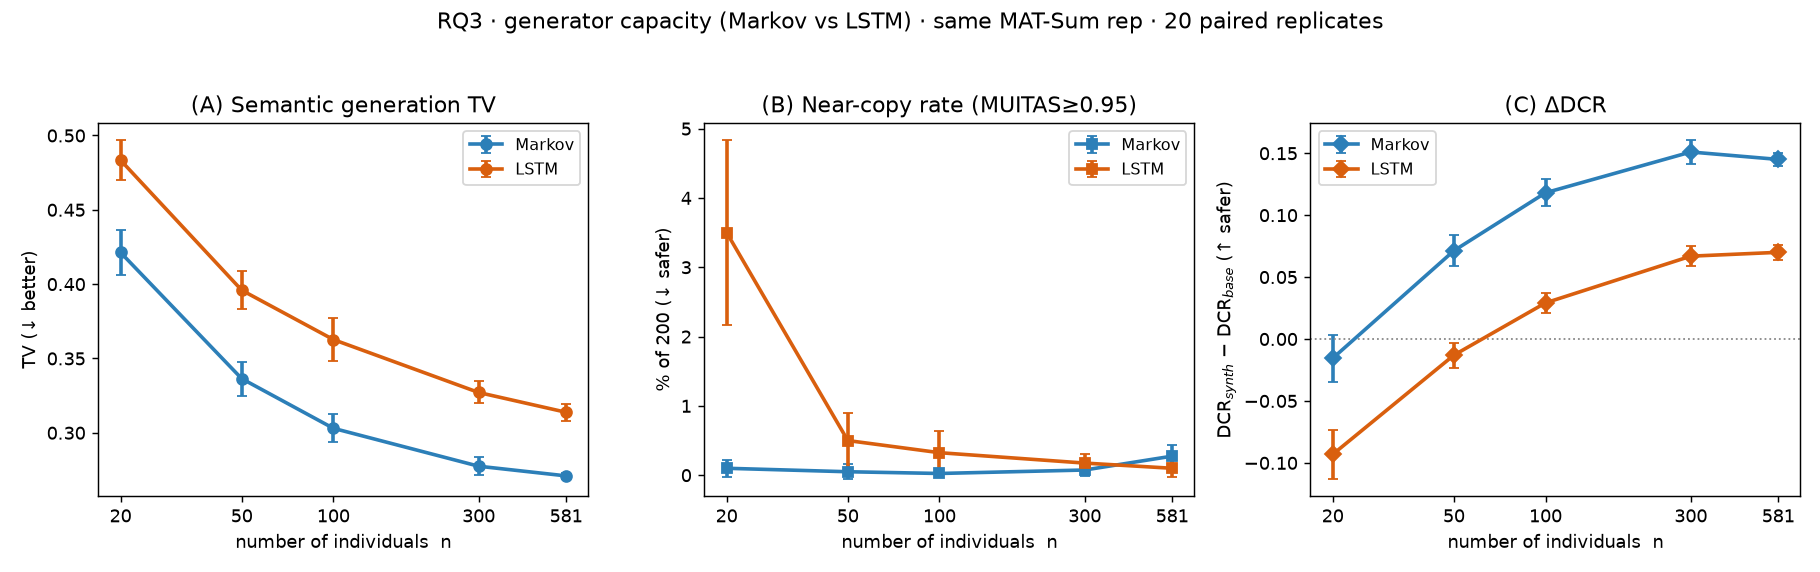
\includegraphics[width=\textwidth]{figures/fig_rq3.png}
  \caption{RQ3 (Paris-581): generator capacity at a fixed \textsc{MAT-Sum} representation, over the
  same 20 nested paired user samples as RQ2 ($m{=}2,k{=}5$; identical length and dwell models;
  $N{=}200$ synthetic/run). \textbf{(A)}~the order-1 Markov attains better semantic fidelity than the
  LSTM at every $n$; \textbf{(B)}~the LSTM's near-copy rate (max training MUITAS $\ge0.95$) is higher,
  acutely at small $n$; \textbf{(C)}~the Markov's $\Delta$DCR is higher (safer) throughout. Means
  $\pm$ 95\% CI.}
  \label{fig:rq3}
\end{figure*}

\begin{table}[t]
  \caption{RQ3: generator capacity at a fixed \textsc{MAT-Sum} representation (Paris-581, 20 nested
  paired replicates). Mean $\pm$ 95\% CI. $\Delta$DCR $=\mathrm{DCR}_{\text{synth}}-\mathrm{DCR}_{\text{base}}$;
  near-copies use max training MUITAS $\ge0.95$; copies out of $N{=}200$.}
  \label{tab:rq3}
  \small
  \begin{tabular}{@{}rlcccc@{}}
    \toprule
    $n$ & model & sem.\ gen-TV\,$\downarrow$ & near-copy \%\,$\downarrow$ & $\Delta$DCR\,$\uparrow$ & exact/200 \\
    \midrule
    \multirow{2}{*}{20}  & Markov & $\mathbf{0.421\pm0.015}$ & $\mathbf{0.10\pm0.12}$ & $\mathbf{-0.015\pm0.019}$ & $0.00$ \\
                         & LSTM   & $0.483\pm0.013$ & $3.50\pm1.33$ & $-0.093\pm0.020$ & $0.40$ \\
    \midrule
    \multirow{2}{*}{50}  & Markov & $\mathbf{0.336\pm0.011}$ & $\mathbf{0.05\pm0.10}$ & $\mathbf{+0.071\pm0.013}$ & $0.10$ \\
                         & LSTM   & $0.396\pm0.013$ & $0.50\pm0.39$ & $-0.013\pm0.010$ & $0.25$ \\
    \midrule
    \multirow{2}{*}{100} & Markov & $\mathbf{0.303\pm0.009}$ & $\mathbf{0.03\pm0.05}$ & $\mathbf{+0.118\pm0.011}$ & $0.00$ \\
                         & LSTM   & $0.363\pm0.014$ & $0.33\pm0.32$ & $+0.029\pm0.008$ & $0.10$ \\
    \midrule
    \multirow{2}{*}{300} & Markov & $\mathbf{0.278\pm0.006}$ & $0.07\pm0.09$ & $\mathbf{+0.151\pm0.010}$ & $0.05$ \\
                         & LSTM   & $0.327\pm0.007$ & $0.17\pm0.14$ & $+0.067\pm0.008$ & $0.05$ \\
    \midrule
    \multirow{2}{*}{581} & Markov & $\mathbf{0.271\pm0.002}$ & $0.28\pm0.16$ & $\mathbf{+0.145\pm0.005}$ & $0.10$ \\
                         & LSTM   & $0.314\pm0.006$ & $0.10\pm0.12$ & $+0.070\pm0.006$ & $0.10$ \\
    \bottomrule
  \end{tabular}
\end{table}


\begin{table}[t]
  \caption{RQ3 (Paris, Markov vs.\ LSTM, 20 nested paired replicates). Mean $\pm$ 95\% CI.
  The LSTM improves the higher-order (trigram) fidelity but degrades first-order (bigram)
  fidelity and---see Table/Fig.\ in Sec.~\ref{sec:rq3}---record-level disclosure. Best
  first-order value per $n$ in bold.}
  \label{tab:rq3-trigram}
  \small
  \begin{tabular}{@{}clcc@{}}
    \toprule
    $n$ & gen. & sem.\ bigram TV\,$\downarrow$ & sem.\ trigram TV\,$\downarrow$ \\
    \midrule
    \multirow{2}{*}{20}  & Markov & $\mathbf{0.424{\pm}0.014}$ & $0.709{\pm}0.017$ \\
                         & LSTM   & $0.483{\pm}0.013$ & $0.692{\pm}0.014$ \\
    \midrule
    \multirow{2}{*}{50}  & Markov & $\mathbf{0.335{\pm}0.011}$ & $0.647{\pm}0.013$ \\
                         & LSTM   & $0.396{\pm}0.013$ & $0.610{\pm}0.011$ \\
    \midrule
    \multirow{2}{*}{100} & Markov & $\mathbf{0.305{\pm}0.009}$ & $0.615{\pm}0.009$ \\
                         & LSTM   & $0.363{\pm}0.014$ & $0.569{\pm}0.012$ \\
    \midrule
    \multirow{2}{*}{300} & Markov & $\mathbf{0.278{\pm}0.005}$ & $0.581{\pm}0.005$ \\
                         & LSTM   & $0.327{\pm}0.007$ & $0.533{\pm}0.005$ \\
    \midrule
    \multirow{2}{*}{581} & Markov & $\mathbf{0.273{\pm}0.003}$ & $0.568{\pm}0.002$ \\
                         & LSTM   & $0.314{\pm}0.006$ & $0.524{\pm}0.004$ \\
    \bottomrule
  \end{tabular}
\end{table}



\subsubsection*{External replication (GeoLife)}
\label{sec:geolife-e3}

We evaluate the privacy–fidelity trade-off induced by generator capacity while holding the semantic representation fixed. On the same nested GeoLife samples used above, we compare the order-1 Markov generator with a lightweight LSTM using the same per-sample MAT-Sum vocabulary and the same session-length and dwell-time models. The LSTM uses an embedding size of 32, a hidden size of 64, and a single recurrent layer, with user-balanced, length-capped, minibatched training. The comparison is performed for n$\in$\{20,50,100,152\}, with 20 paired replicates and N=200 synthetic sessions per run. We report the semantic bigram TV, the semantic trigram TV, the near-copy rate, the exact copies, and user-aware $\Delta$DCR.


On the same MAT-Sum representation and the same nested paired user samples as
Section~\ref{sec:geolife-e2}, we compare the order-1 Markov generator with a light LSTM
(embedding $32$, hidden $64$, one layer; user-balanced, length-capped, minibatched training),
for $n\in\{20,50,100,152\}$ over $20$ nested paired replicates. We report first-order semantic
fidelity (label bigram TV), higher-order fidelity (label trigram TV), record-level disclosure
(near-copy rate: \% synthetic sessions with maximum training MUITAS $\ge 0.95$; exact copies),
and the user-aware $\Delta$DCR (Table~\ref{tab:geolife-e3}, Figure~\ref{fig:geolife-e3}).
The Paris RQ3 finding replicates. The Markov provides better first-order semantic fidelity and lower empirical disclosure risk, whereas the LSTM captures higher-order sequential structure more accurately at the cost of greater proximity to training records. Its bigram TV is lower---and the gap \emph{widens} with $n$
(paired sign-flip test, Markov$-$LSTM $=-0.021$, $p{=}0.025$ at $n{=}20$; $-0.044$, $p{<}10^{-4}$
at $n{=}152$)---while its near-copy rate stays near zero against the LSTM's $6.5\%$ at $n{=}20$
($p{<}10^{-4}$), and its $\Delta$DCR is positive throughout whereas the LSTM is negative at
$n{=}20$ ($-0.053\pm0.012$, i.e.\ synthetic sessions closer to training than reals are to each
other) and below Markov everywhere. The one axis on which the LSTM wins is the trigram TV
($\approx0.49$ vs.\ $\approx0.59$): its extra capacity does capture higher-order sequential
structure the memoryless chain cannot. In these small-data regimes, however, that capacity
surfaces mainly as memorization---worse first-order fidelity, more near-copies, lower
$\Delta$DCR---rather than a robust fidelity gain. For privacy-preserving synthesis the
interpretable order-1 Markov is therefore the better operating point, externally confirming RQ3.

\begin{table*}[t]
  \caption{GeoLife (RQ3; Markov vs.\ LSTM, 20 nested paired replicates). Mean $\pm$ 95\% CI;
  near-copy $=\%$ synthetic with max training MUITAS $\ge0.95$; copies out of $200$;
  $\Delta$DCR user-aware. Best (privacy-relevant) value per $n$ in bold.}
  \label{tab:geolife-e3}
  \small
  \setlength{\tabcolsep}{4pt}
  \begin{tabular}{@{}clccccc@{}}
    \toprule
    $n$ & gen. & bi-TV\,$\downarrow$ & tri-TV\,$\downarrow$ & near-copy\%\,$\downarrow$ & exact & $\Delta$DCR\,$\uparrow$ \\
    \midrule
    \multirow{2}{*}{20}  & Markov & $\mathbf{0.287{\pm}0.019}$ & $0.591{\pm}0.015$ & $\mathbf{0.42{\pm}0.47}$ & $0.0$ & $\mathbf{+0.010{\pm}0.013}$ \\
                         & LSTM   & $0.308{\pm}0.020$ & $\mathbf{0.490{\pm}0.020}$ & $6.47{\pm}1.51$ & $0.6$ & $-0.053{\pm}0.012$ \\
    \midrule
    \multirow{2}{*}{50}  & Markov & $\mathbf{0.282{\pm}0.013}$ & $0.596{\pm}0.011$ & $\mathbf{0.78{\pm}0.54}$ & $0.0$ & $\mathbf{+0.029{\pm}0.009}$ \\
                         & LSTM   & $0.290{\pm}0.013$ & $\mathbf{0.489{\pm}0.012}$ & $2.35{\pm}0.78$ & $0.1$ & $-0.002{\pm}0.007$ \\
    \midrule
    \multirow{2}{*}{100} & Markov & $\mathbf{0.268{\pm}0.006}$ & $0.584{\pm}0.006$ & $\mathbf{0.42{\pm}0.52}$ & $0.0$ & $\mathbf{+0.034{\pm}0.007}$ \\
                         & LSTM   & $0.294{\pm}0.013$ & $\mathbf{0.491{\pm}0.010}$ & $1.27{\pm}0.45$ & $0.1$ & $+0.013{\pm}0.006$ \\
    \midrule
    \multirow{2}{*}{152} & Markov & $\mathbf{0.252{\pm}0.004}$ & $0.568{\pm}0.006$ & $\mathbf{0.25{\pm}0.18}$ & $0.1$ & $\mathbf{+0.034{\pm}0.008}$ \\
                         & LSTM   & $0.295{\pm}0.008$ & $\mathbf{0.495{\pm}0.008}$ & $0.93{\pm}0.44$ & $0.2$ & $+0.022{\pm}0.006$ \\
    \bottomrule
  \end{tabular}
\end{table*}

\begin{figure*}[t]
  \centering
  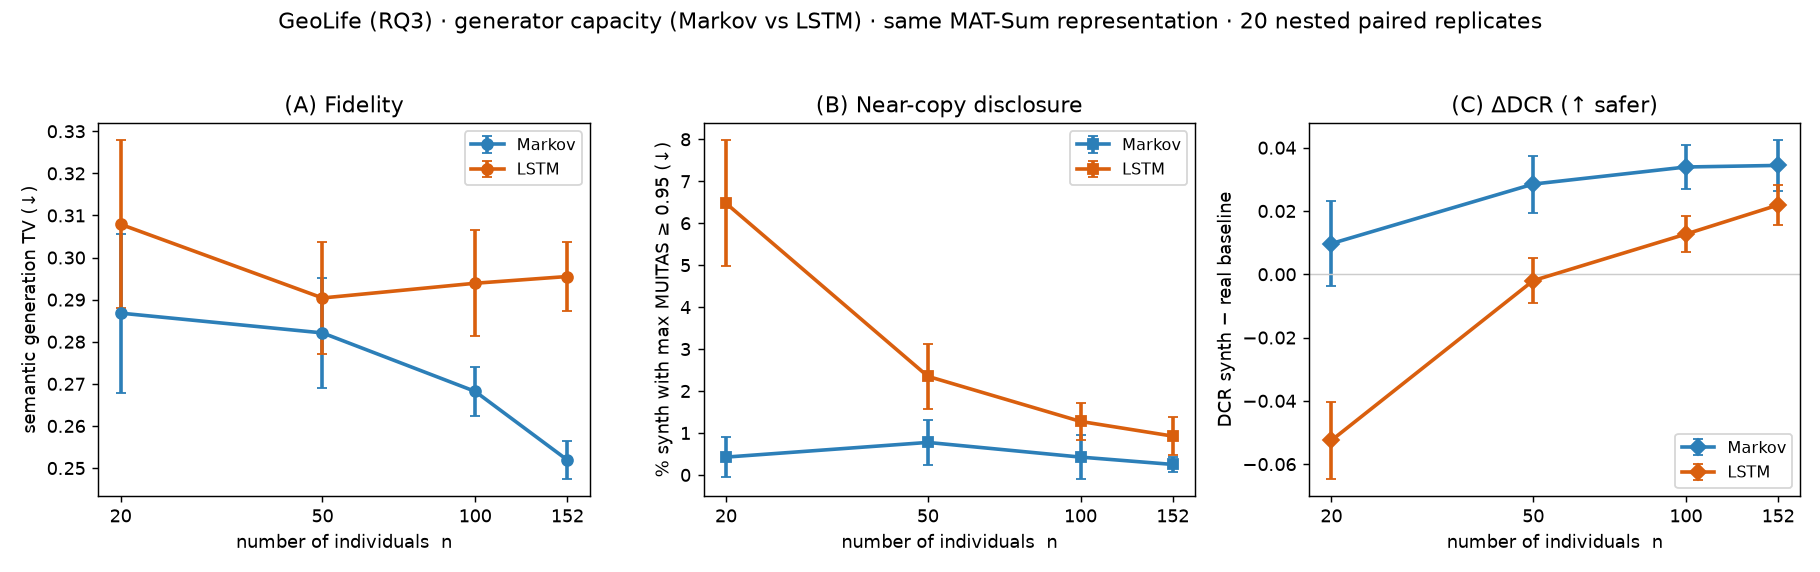
\includegraphics[width=\textwidth]{figures/geolife_e3.png}
  \caption{GeoLife (RQ3) generator capacity, 20 nested paired replicates. \textbf{(A)}~first-order
  semantic fidelity (bigram TV): Markov lower at every $n$, gap widening; \textbf{(B)}~near-copy
  disclosure: the LSTM leaks markedly at small $n$; \textbf{(C)}~user-aware $\Delta$DCR: Markov
  positive throughout, the LSTM negative at $n{=}20$. Means $\pm$ 95\% CI.}
  \label{fig:geolife-e3}
\end{figure*}


The two generators occupy different positions on the privacy–fidelity frontier. The Markov model consistently achieves lower semantic bigram TV, with the gap increasing from 0.021 at n=20 to 0.043 at n=152. By contrast, the LSTM consistently achieves lower trigram TV—approximately 0.49, compared with 0.57–0.60 for the Markov—showing that its additional capacity captures higher-order sequential dependencies that an order-1 process cannot model directly. Thus, the LSTM provides a genuine gain in higher-order fidelity, rather than a uniformly inferior reconstruction of the data.

This higher-order gain is accompanied by a substantially less favorable disclosure profile, especially when users are scarce. At n=20, the LSTM produces a 6.47\% near-copy rate, compared with 0.42\% for the Markov, and its $\Delta$DCR is negative (−0.053), whereas the Markov remains slightly positive (+0.010). The disclosure gap narrows as n increases, but the Markov retains the higher $\Delta$DCR and lower near-copy rate across the evaluated regimes. These findings indicate that higher model capacity can recover longer-range structure, but at the cost of greater proximity to individual training records in the small-data regime.

For the target application of generating shareable mobility data from small datasets, the order-1 Markov therefore represents the more conservative operating point: it sacrifices some higher-order fidelity while providing better first-order distributional fidelity and consistently lower empirical disclosure risk. The LSTM remains useful as evidence that model capacity changes the nature of the fidelity being preserved, but its advantages should be assessed jointly with the associated memorization cost rather than through fidelity alone.

Overall, the GeoLife experiments confirm the three central findings of the paper. First, semantic abstraction produces a more faithful and learnable generative representation than matched geometric alternatives. Second, the value of additional users depends on the amount of mobility information contributed by each individual, rather than on population size alone. Third, generator capacity introduces a genuine privacy–fidelity trade-off: higher-capacity models recover more higher-order structure, while simpler mechanistic generation provides a more favourable empirical disclosure profile in the small-data regimes that motivate the work.

\subsection{What generalizes across datasets}
\label{sec:cross}

The external validation reveals both stable findings and dataset-dependent scaling effects. Across Paris-OSM and GeoLife, MAT-Sum consistently provides a more faithful and learnable generative representation than matched geometric abstractions, confirming that the advantage originates from the semantic construction of the state space rather than from a particular city or collection process. The scaling behaviour, however, differs between datasets: quality improves substantially with the number of individuals on Paris, whereas GeoLife is already informative at small n because each user contributes multiple semantically rich sessions. This indicates that the effective sample size depends on both the number of individuals and the amount of mobility information contributed per individual.

Generator capacity also produces a consistent privacy–fidelity tension. The order-1 Markov provides better first-order semantic fidelity and a more favorable empirical disclosure profile, particularly when training users are scarce. The LSTM captures higher-order sequential structure more accurately on GeoLife, but this gain is accompanied by higher near-copy rates and lower $\Delta$DCR. Taken together, the two datasets support semantic abstraction and low-capacity mechanistic generation as a conservative operating point for synthesis from small confidential mobility datasets.


\section{Privacy and utility of the released data}
\label{sec:privacy-utility}

\subsection{Utility: train-on-synthetic, test-on-real (TSTR)}
\label{sec:tstr}
To close the utility leg of the triad we evaluate a downstream task---next-semantic-label
prediction in the fixed OSM-label space. A fixed 20\% of individuals is held out as a real test
set; a predictor is fit either on the real training individuals (TRTR, upper bound) or on the
synthetic data (TSTR), and scored as top-1 accuracy on the real test set; a majority-label
predictor is the lower bound. We report the utility retained,
$(\mathrm{TSTR}-\mathrm{base})/(\mathrm{TRTR}-\mathrm{base})$, for an order-1 and an order-2
predictor (Table~\ref{tab:tstr}, Figure~\ref{fig:tstr}). The synthetic data retains
$\approx\!80\%$ of the first-order predictive signal at every $n$, providing direct evidence that
it supports a real analysis task and not merely distributional matching. The second-order utility,
however, is largely lost ($\approx\!25\%$ retained): the memoryless generator cannot reproduce the
higher-order structure that a second-order predictor exploits (real second-order accuracy nearly
doubles the first-order one). This connects RQ3 to utility: the higher-order structure the LSTM
recovers (its trigram advantage) carries genuine downstream value, so generator capacity trades
not only fidelity but utility against disclosure.

\begin{table}[t]
  \caption{TSTR on Paris-581: next-label top-1 accuracy on a held-out real test set (mean over
  20 replicates). ``retained'' $=(\mathrm{TSTR}-\mathrm{base})/(\mathrm{TRTR}-\mathrm{base})$.}
  \label{tab:tstr}
  \small
  \begin{tabular}{@{}rccccccc@{}}
    \toprule
     & & \multicolumn{3}{c}{order-1} & \multicolumn{2}{c}{order-2} \\
    \cmidrule(lr){3-5}\cmidrule(lr){6-7}
    $n$ & base & TRTR & TSTR & retained & TRTR & TSTR/ret. \\
    \midrule
    20  & 0.144 & 0.195 & 0.182 & $0.81$ & 0.323 & $0.30$ \\
    50  & 0.145 & 0.210 & 0.195 & $0.82$ & 0.388 & $0.26$ \\
    100 & 0.144 & 0.219 & 0.202 & $0.79$ & 0.424 & $0.25$ \\
    300 & 0.143 & 0.229 & 0.213 & $0.82$ & 0.465 & $0.27$ \\
    465 & 0.143 & 0.231 & 0.217 & $0.84$ & 0.473 & $0.25$ \\
    \bottomrule
  \end{tabular}
\end{table}

\begin{figure}[t]\centering
  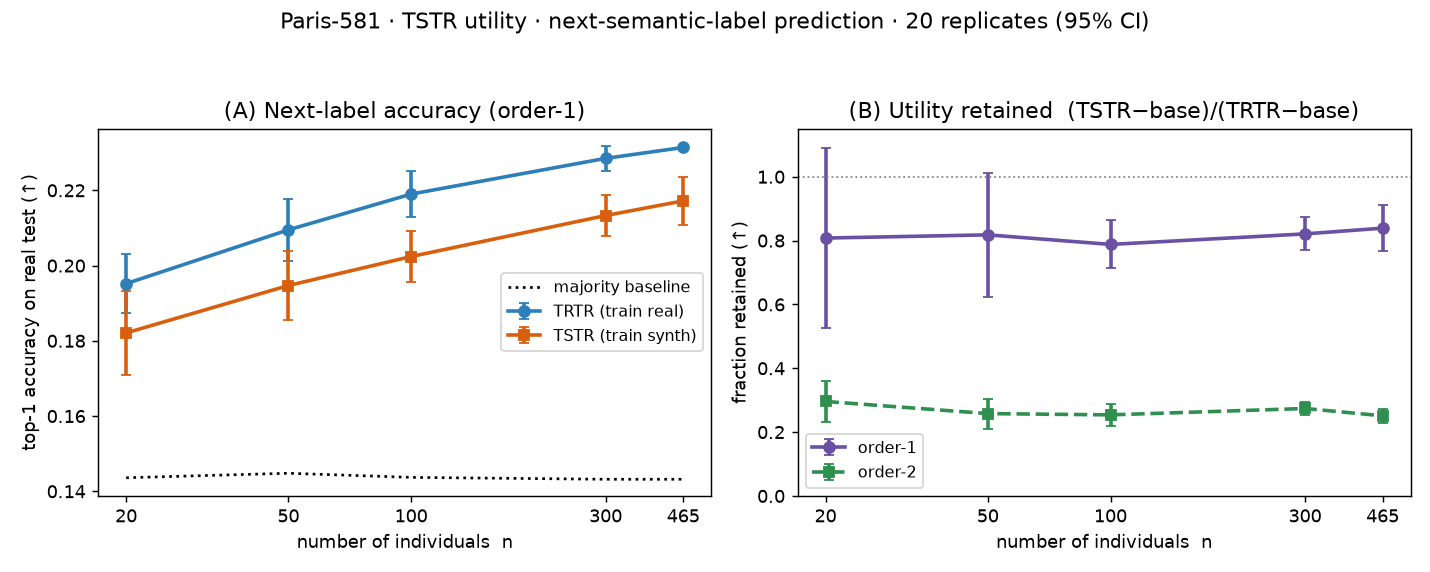
\includegraphics[width=\columnwidth]{figures/paris_tstr.png}
  \caption{TSTR utility on Paris-581. (A) next-label accuracy: TSTR tracks TRTR well above the
  majority baseline (order-1). (B) utility retained: $\approx\!80\%$ at order-1, $\approx\!25\%$
  at order-2. Means $\pm$ 95\% CI.}
  \label{fig:tstr}
\end{figure}

\subsection{Worst-case disclosure: near-copy threshold sweep and DCR tail}
\label{sec:disclosure-tail}
Mean $\Delta$DCR summarises the average record; disclosure risk, however, lives in the tail. We
therefore report (i) the near-copy rate as a function of the threshold $\tau\in[0.80,1.0]$, against
a real-to-real baseline (each real record vs.\ all other real records; user-aware on GeoLife), and
(ii) the tail of the DCR distribution (Figures~\ref{fig:disc-paris}--\ref{fig:disc-geo}). On both
datasets the synthetic near-copy rate lies \emph{below the real-to-real similarity floor at every
threshold}: at $\tau{=}0.95$ it is $0.08$--$0.63\%$ on Paris and $1.6$--$2.2\%$ on GeoLife, against
real-to-real baselines of $4.5$--$27\%$ and $4.9$--$26\%$ respectively---synthetic records are no
closer to the training set than real records already are to one another. The fifth-percentile DCR
stays well positive ($0.11$--$0.20$ on Paris, $0.07$--$0.08$ on GeoLife). The minimum DCR is $0$ at
all $n$, but this reflects the set-based, order-insensitive nature of MUITAS (similarity $1$ without
verbatim identity): exact sequence copies remain $\le 0.1$ per $200$. The only regime where the
synthetic rate marginally exceeds the real baseline is the smallest sample at the strictest
threshold (GeoLife $n{=}10$, $\tau{=}1.0$: $0.075\%$ vs.\ $0.039\%$), consistent with the mildly
negative $\Delta$DCR reported there.

\begin{figure}[t]\centering
  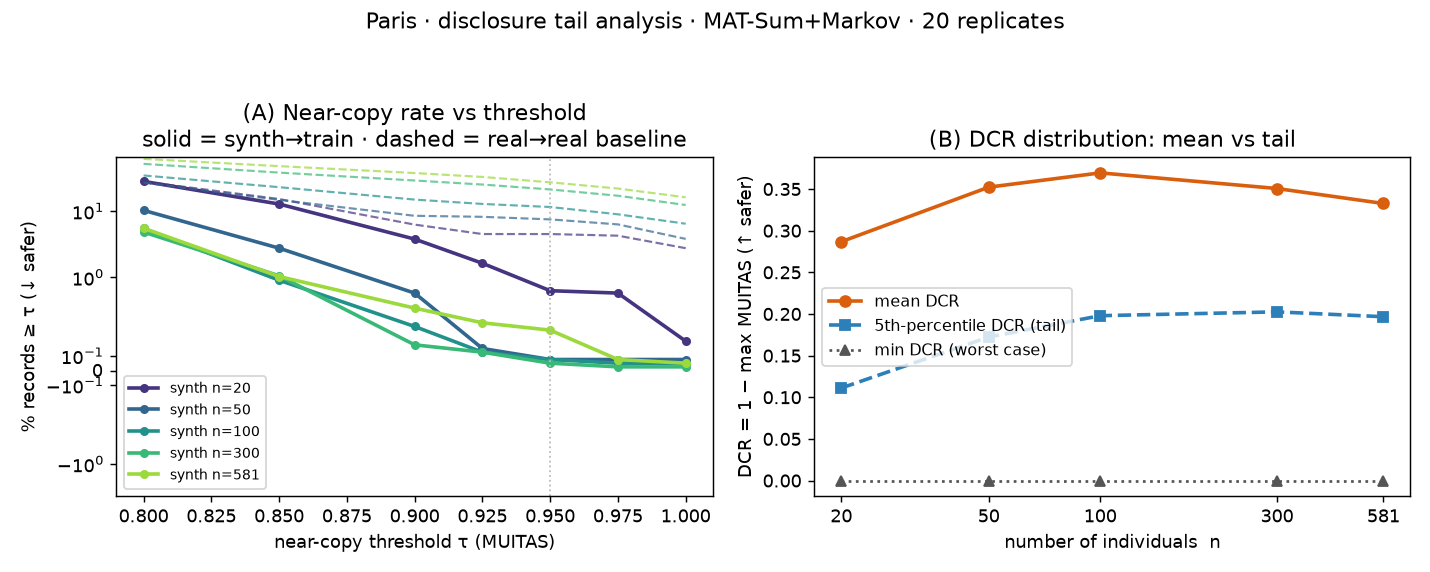
\includegraphics[width=\columnwidth]{figures/Paris_disclosure.png}
  \caption{Paris-581 disclosure tail. (A) near-copy rate vs.\ threshold: synthetic (solid) far
  below the real-to-real baseline (dashed) at every $\tau$. (B) DCR mean vs.\ tail.}
  \label{fig:disc-paris}
\end{figure}
\begin{figure}[t]\centering
  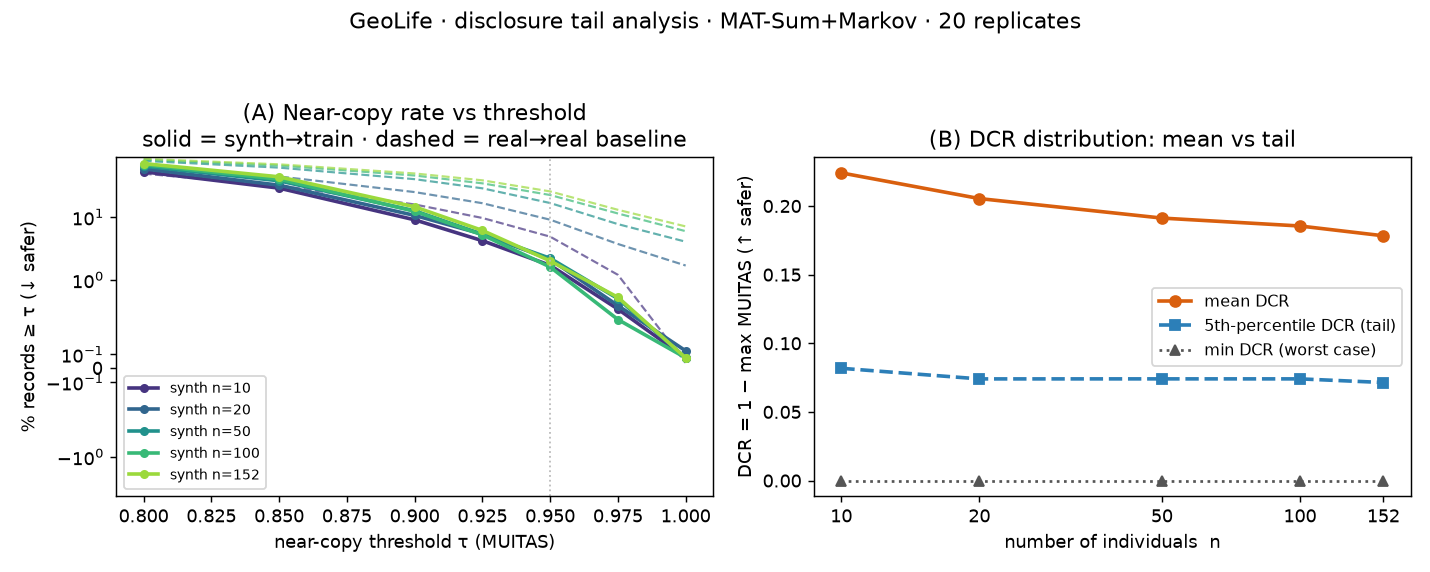
\includegraphics[width=\columnwidth]{figures/GeoLife_disclosure.png}
  \caption{GeoLife disclosure tail (user-aware baseline); same reading as Fig.~\ref{fig:disc-paris}.}
  \label{fig:disc-geo}
\end{figure}

\subsection{Privacy analysis: membership inference and unicity}
\label{sec:privacy-attacks}
Beyond the copy/DCR measures, we complete the privacy triad with a membership-inference attack and a
unicity analysis. \textbf{Membership inference.} We mount the standard distance-to-closest-record
attack against the released synthetic set: a candidate real record $x$ is scored by
$s(x)=\max_j \mathrm{MUITAS}(x,\tilde s_j)$ and predicted a training member when $s(x)$ is high. We
report the ROC-AUC of separating true members (the $n$ training records) from a fixed held-out set of
non-members (20\% of individuals on Paris, of users on GeoLife), and the TPR at $10\%$ FPR
(Table~\ref{tab:mia}, Figure~\ref{fig:mia}). The attack essentially fails: the AUC is indistinguishable
from chance ($0.5$) at all sample sizes and drops below it as $n$ grows (members are no closer to the
synthetic data than non-members). The only---weak---advantage appears at the smallest sample
($n{=}20$ on Paris: AUC $0.547$, TPR@10\% $0.134$) and vanishes by $n{=}50$, consistent with the mildly
negative $\Delta$DCR reported there. This is a black-box distance attack; a shadow-model attack is left
to future work. \textbf{Unicity.} Following the ``unique in the crowd'' methodology in the semantic
space, we draw $k$ labels from a record and call it unique-at-$k$ when a single dataset record contains
all $k$. Synthetic records are $10$--$20\times$ less identifiable than real ones (e.g.\ at $k{=}4$,
$0.08\%$ vs.\ $1.5\%$ on Paris and $0.17\%$ vs.\ $2.1\%$ on GeoLife; Figure~\ref{fig:unicity}). Notably,
even the real data has low unicity at the semantic granularity, i.e.\ the abstraction is itself less
identifying than raw GPS traces, and the synthetic release lowers it further.

\begin{table}[t]
  \caption{Membership inference (distance-to-closest-synthetic, 20 replicates, mean $\pm$ 95\% CI).
  AUC $=0.5$ and TPR$=0.10$ at $10\%$ FPR indicate no membership signal.}
  \label{tab:mia}
  \small
  \begin{tabular}{@{}rcccc@{}}
    \toprule
     & \multicolumn{2}{c}{Paris-581} & \multicolumn{2}{c}{GeoLife} \\
    \cmidrule(lr){2-3}\cmidrule(lr){4-5}
    $n$ & AUC & TPR@10\% & AUC & TPR@10\% \\
    \midrule
    20  & $0.547{\pm}.023$ & $0.134$ & $0.478{\pm}.015$ & $0.076$ \\
    50  & $0.506{\pm}.017$ & $0.100$ & $0.483{\pm}.017$ & $0.126$ \\
    100 & $0.491{\pm}.012$ & $0.074$ & $0.469{\pm}.012$ & $0.125$ \\
    300/121 & $0.474{\pm}.006$ & $0.076$ & $0.465{\pm}.011$ & $0.124$ \\
    465 & $0.476{\pm}.006$ & $0.076$ & -- & -- \\
    \bottomrule
  \end{tabular}
\end{table}

\begin{table}[t]
  \caption{Unicity: \% of records uniquely identified by $k$ random semantic labels (real vs.\ same-size synthetic).}
  \label{tab:unicity}
  \small
  \begin{tabular}{@{}ccccc@{}}
    \toprule
     & \multicolumn{2}{c}{Paris-581} & \multicolumn{2}{c}{GeoLife} \\
    \cmidrule(lr){2-3}\cmidrule(lr){4-5}
    $k$ & real & synth & real & synth \\
    \midrule
    1 & $0.055$ & $0.000$ & $0.016$ & $0.000$ \\
    2 & $0.336$ & $0.000$ & $0.140$ & $0.004$ \\
    3 & $0.657$ & $0.007$ & $0.781$ & $0.032$ \\
    4 & $1.545$ & $0.081$ & $2.136$ & $0.169$ \\
    \bottomrule
  \end{tabular}
\end{table}

\begin{figure}[t]\centering
  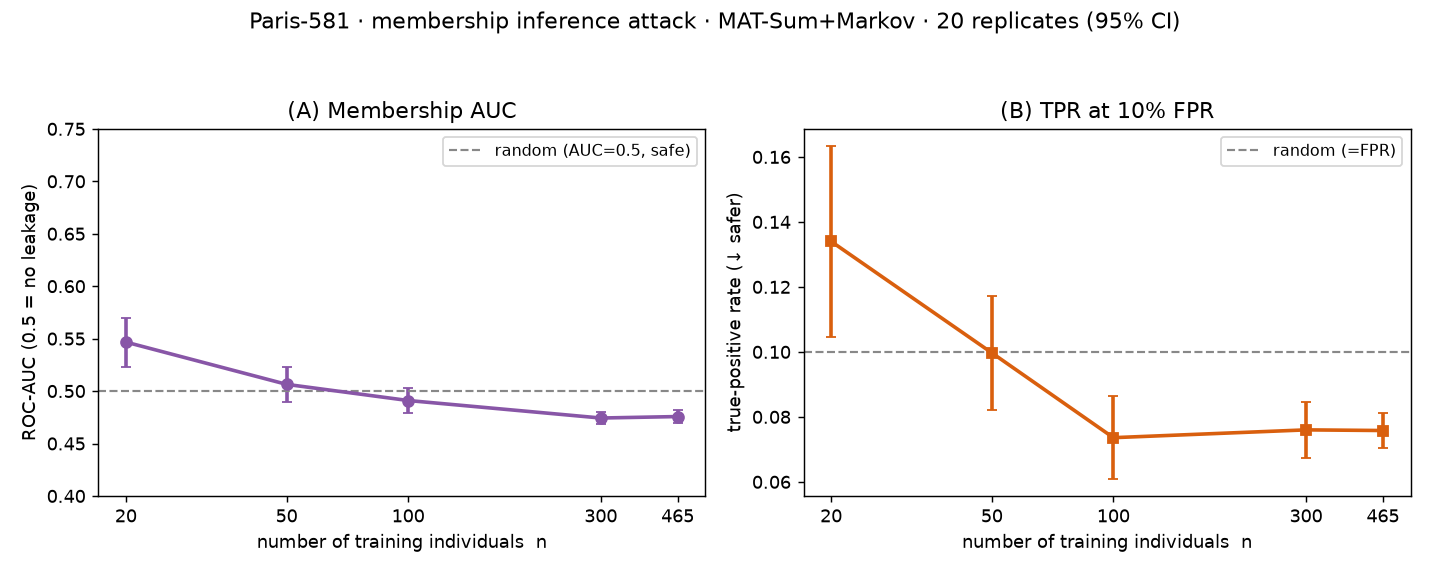
\includegraphics[width=\columnwidth]{figures/paris_mia.png}
  \caption{Membership inference on Paris-581: AUC near/below $0.5$ (A) and TPR@10\%FPR near the random
  line (B); a weak signal only at $n{=}20$. GeoLife (Table~\ref{tab:mia}) shows no signal at any $n$.}
  \label{fig:mia}
\end{figure}
\begin{figure}[t]\centering
  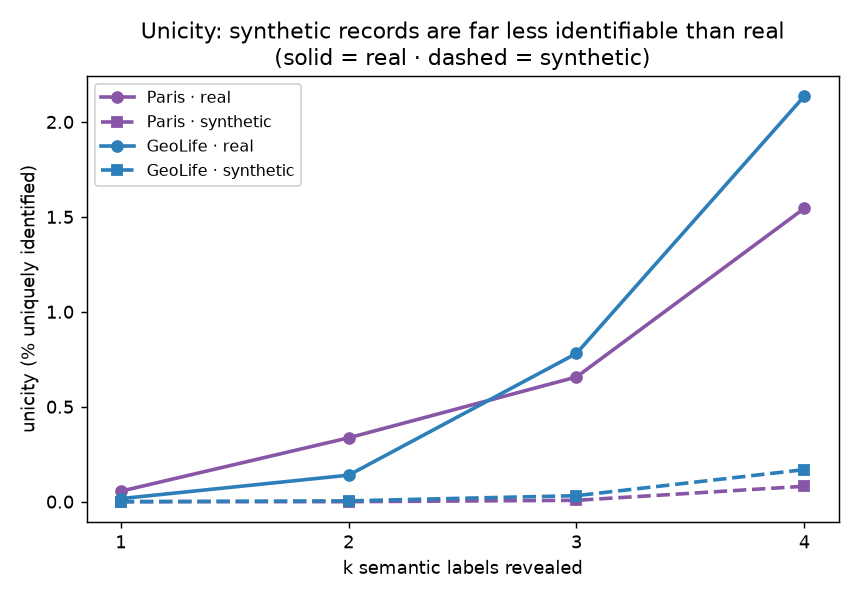
\includegraphics[width=\columnwidth]{figures/unicity_combined.png}
  \caption{Unicity vs.\ $k$: synthetic records (dashed) are $10$--$20\times$ less identifiable than real
  ones (solid) on both datasets.}
  \label{fig:unicity}
\end{figure}


\section{Conclusions and Future works}

In this work, we investigated how to generate synthetic semantic mobility data from a small, potentially confidential dataset.
Our central idea is to use MAT-Sum not only as a summarization method, but as the representation on which generation takes place. MAT-Sum transforms mobility into sequences over semantically characterized
locations, providing a meaningful generative state space rather than operating directly on coordinates or purely geometric regions.

Our experiments show that this choice of representation matters.
When state-space size and sequence generator are controlled, MAT-Sum introduces less semantic distortion and yields a transition space that is reproduced more accurately than matched grid and spatial-clustering
representations. The scaling experiments further show that semantic generation remains viable in small-data regimes and improves as more mobility information becomes available, while empirical record-level
memorization remains limited. Finally, increasing generator capacity does not provide a uniform advantage: the LSTM captures higher-order
sequential dependencies more accurately, whereas the order-1 Markov model provides better first-order fidelity and a more conservative empirical disclosure profile when training data are scarce.

A dedicated privacy analysis, exact and near-copy rates, the tail of the distance-to-closest-record
distribution against a real-to-real baseline, a membership-inference attack, and a unicity study, shows
that record-level disclosure stays limited on both datasets: synthetic records are no closer to the
training data than real records are to one another, the membership attack performs no better than chance
(AUC $\approx 0.5$) beyond the smallest sample, and synthetic records are an order of magnitude less
uniquely identifiable than real ones.

Taken together, these findings support a representation-first, privacy-aware view of synthetic mobility generation. When the goal is to create a shareable surrogate of a small confidential population,
semantic abstraction can help preserve the mobility information of interest while reducing dependence on individual training records.


As future work, we plan a system-level comparison with recent geometry-centric generation pipelines. Such a comparison requires re-running the approaches under common data, preprocessing, and evaluation conditions, and jointly assessing semantic fidelity,
record-level disclosure, and aggregate spatial fidelity.
A second important direction is to strengthen the privacy analysis. The present work focuses on empirical record-level disclosure through exact and near copies and distance to the closest training records, rather than providing a formal privacy guarantee. Future work will therefore investigate stronger privacy evaluations, including explicit privacy attacks such as membership inference, as well as the possible integration of formal privacy mechanisms such as differential privacy.
Stronger membership attacks (shadow-model and likelihood-ratio), a formal differential-privacy
guarantee on the transition counts, and treating the min-support $k$ as an explicit
privacy--fidelity knob would tighten the privacy characterisation; on utility, higher-order
generators that recover sequential structure without memorising, the geographic re-materialisation
of sequences to GPS, and a system-level comparison against deep, differentially-private, and
mechanistic baselines remain the natural next steps.

%We argued and gave the first evidence that a location-centric semantic summarization, \textsc{MAT-Sum}, is
%a natural substrate for privacy-preserving synthesis of Multiple-Aspect Trajectories. Generating over
%a $k$-anonymized semantic vocabulary yields synthetic mobility that is semantically rich, controllably
%private and data-efficient---a combination no single existing technique offers---and a simple
%mechanistic generator dominates a deep one on the fidelity/privacy trade-off---an interpolated
%variable-order variant improves higher-order fidelity, while a differentially-private variant adds a
%formal guarantee. Natural next steps are cross-city validation (New York), a tuned adaptive-DP
%synthesizer, a TSTR utility study, and a membership-inference audit at scale.

%% ---------------------------------------------------------------------------
%% Self-contained bibliography (replace with a .bib + ACM-Reference-Format for submission).
\begin{thebibliography}{99}
\bibitem{bogorny2019} R.~dos Santos Mello, V.~Bogorny, et al. MASTER: A Multiple Aspect View on Trajectories. \emph{Transactions in GIS}, 2019.
\bibitem{feng2020} J.~Feng, Z.~Yang, et al. Learning to Simulate Human Mobility (MoveSim). \emph{KDD}, 2020.
\bibitem{geolife} Y.~Zheng, X.~Xie, and W.-Y.~Ma. GeoLife: A Collaborative Social Networking Service
among User, Location and Trajectory. \emph{IEEE Data Eng.\ Bull.}, 33(2):32--39, 2010.
\bibitem{gruteser2003} M.~Gruteser and D.~Grunwald. Anonymous Usage of Location-Based Services through Spatial and Temporal Cloaking. \emph{MobiSys}, 2003.
\bibitem{gursoy2018} M.~E.~G\"ursoy, L.~Liu, et al. Utility-Aware Synthesis of Differentially Private and Attack-Resilient Location Traces (AdaTrace). \emph{ACM CCS}, 2018.
\bibitem{kavalionak2026} H.~Kavalionak, C.~Pugliese, E.~Carlini, C.~Renso,
T.~Chevallier, G.~Vangilluwen, and V.~Delmas. Toward a General Graph-Based Abstraction
Approach for Urban Trajectory Generation. \emph{MuseKDE Workshop}, IEEE International Conference on Mobile Data Management, Athens, 2026.
\bibitem{krajzewicz2002} D.~Krajzewicz, G.~Hertkorn, C.~R\"ossel, and P.~Wagner. SUMO
(Simulation of Urban MObility). \emph{Middle East Symp. on Simulation and Modelling}, 2002.
\bibitem{jiang2016} S.~Jiang, Y.~Yang, et al. The TimeGeo Modeling Framework. \emph{PNAS}, 2016.
\bibitem{montjoye2013} Y.-A.~de Montjoye, C.~A.~Hidalgo, et al. Unique in the Crowd: The Privacy Bounds of Human Mobility. \emph{Scientific Reports}, 2013.
\bibitem{pappalardo2018} L.~Pappalardo and F.~Simini. Data-driven Generation of Spatio-temporal Routines in Human Mobility (DITRAS). \emph{Data Mining and Knowledge Discovery}, 2018.
\bibitem{petry2019} L.~M.~Petry, C.~A.~Ferrero, et al. Towards Semantic-Aware Multiple-Aspect Trajectory Similarity Measuring (MUITAS). \emph{IJGIS}, 2019.
\bibitem{pugliese2023} C.~Pugliese, F.~Lettich, F.~Pinelli, C.~Renso. Summarizing Trajectories Using Semantically Enriched Geographical Context (MAT-Sum). \emph{ACM SIGSPATIAL}, 2023.
\bibitem{pugliese2025} C.~Pugliese, F.~Lettich, G.~Rocchietti, C.~Renso, F.~Pinelli. Human Mobility Datasets Enriched With Contextual and Social Dimensions. \emph{arXiv:2510.02333}; Zenodo 15658129, 2025.
\bibitem{privtrace} H.~Wang, Z.~Zhang, et al. PrivTrace: Differentially Private Trajectory Synthesis by Adaptive Markov Models. \emph{USENIX Security}, 2023.
\bibitem{wang2024stdifftraj} B.~Wang, J.~Yu, J.~Han, and S.~Qiu. ST-DiffTraj: A Spatiotemporal-Aware Diffusion Model for Trajectory Generation. In \emph{Proc.\ 7th Int.\ Conf.\ on Algorithms, Computing and Artificial Intelligence (ACAI)}, 2024.
\bibitem{rao2020} J.~Rao, S.~Gao, et al. LSTM-TrajGAN: A Deep Learning Approach to Trajectory Privacy Protection. \emph{GIScience}, 2020.
\bibitem{song2010} C.~Song, T.~Koren, P.~Wang, A.-L.~Barab\'asi. Modelling the Scaling Properties of Human Mobility (EPR). \emph{Nature Physics}, 2010.
\bibitem{spaccapietra2008} S.~Spaccapietra, C.~Parent, et al. A Conceptual View on Trajectories. \emph{Data \& Knowledge Engineering}, 2008.
\bibitem{zhu2023} Y.~Zhu, Y.~Ye, et al. DiffTraj: Generating GPS Trajectory with Diffusion Probabilistic Model. \emph{NeurIPS}, 2023.
\bibitem{zuefle_pol} J.-S.~Kim, H.~Kavak, A.~Crooks, D.~Pfoser, C.~Wenk, and A.~Z\"ufle. Location-based social network data generation based on patterns of life. \emph{IEEE MDM}, 2020.

\bibitem{zhu2023difftraj}
Y. Zhu, Y. Ye, S. Zhang, X. Zhao, and J. J. Q. Yu.
DiffTraj: Generating GPS Trajectory with Diffusion Probabilistic Model.
In \emph{Advances in Neural Information Processing Systems (NeurIPS)},
vol. 36, pp. 65168--65188, 2023.

\bibitem{zhu2023synmob}
Y. Zhu, Y. Ye, Y. Wu, X. Zhao, and J. J. Q. Yu.
SynMob: Creating High-Fidelity Synthetic GPS Trajectory Dataset for
Urban Mobility Analysis.
In \emph{Advances in Neural Information Processing Systems (NeurIPS)},
vol. 36, Datasets and Benchmarks Track, pp. 22961--22977, 2023.

\bibitem{zhang2025codiffmob}
Y. Zhang, Y. Yuan, J. Ding, J. Yuan, and Y. Li.
Noise Matters: Diffusion Model-based Urban Mobility Generation with
Collaborative Noise Priors.
In \emph{Proceedings of the ACM Web Conference 2025 (WWW '25)},
pp. 5352--5363, 2025.
doi: 10.1145/3696410.3714516.

\bibitem{dirmeier2024categorical}
S. Dirmeier, Y. Hong, and F. Perez-Cruz.
Synthetic Location Trajectory Generation Using Categorical Diffusion Models.
\emph{arXiv preprint arXiv:2402.12242}, 2024.

\bibitem{fang2025memorization}
Z. Fang, Z. Jiang, H. Chen, X. Li, and J. Li.
Understanding and Mitigating Memorization in Diffusion Models for
Tabular Data.
In \emph{Proceedings of the 42nd International Conference on Machine
Learning (ICML)}, Proceedings of Machine Learning Research,
vol. 267, pp. 15976--16005, 2025.

\end{thebibliography}

\end{document}
